%!TeX root = 5-diffusion.tex
\documentclass[main]{subfiles}

\begin{document}

\chapter{Xenon and krypton transport properties}
\vspace*{-1\baselineskip}


In separation processes, diffusion can either be the main performance metric or a neglected secondary parameter. There are actually two different use cases for separation using nanoporous materials: the adsorption-based separation that is mainly a thermodynamic process and the nanoporous separation membranes that relies on the kinetic properties. In a membrane-based process, the gas is sieved through a membrane material that blocks some molecules (e.g. Xe) and let other molecules (e.g.) diffuse freely. The performance of the separation is measured with the ratio of the diffusion coefficients instead of the thermodynamic selectivity I defined in chapter 2. The process of interest is, however, the adsorption-based separation performed industrially by pressure and/or temperature swing adsorption, and even if the thermodynamic selectivity is the main performance metric, the kinetic performances can improve the overall indstrial process.\autocite{Kumar_1994} For instance, in breakthrough experiments (a lab equivalent of a pressure swing adsorption) used to characterize the comparative adsorption performances of a gas mixture, the shape of the curve can be explained by diffusion processes. The goal of this chapter is to explore this often neglected diffusion parameter in an adsorption-based Xe/Kr separation process.

\begin{figure}[ht]
  \centering
    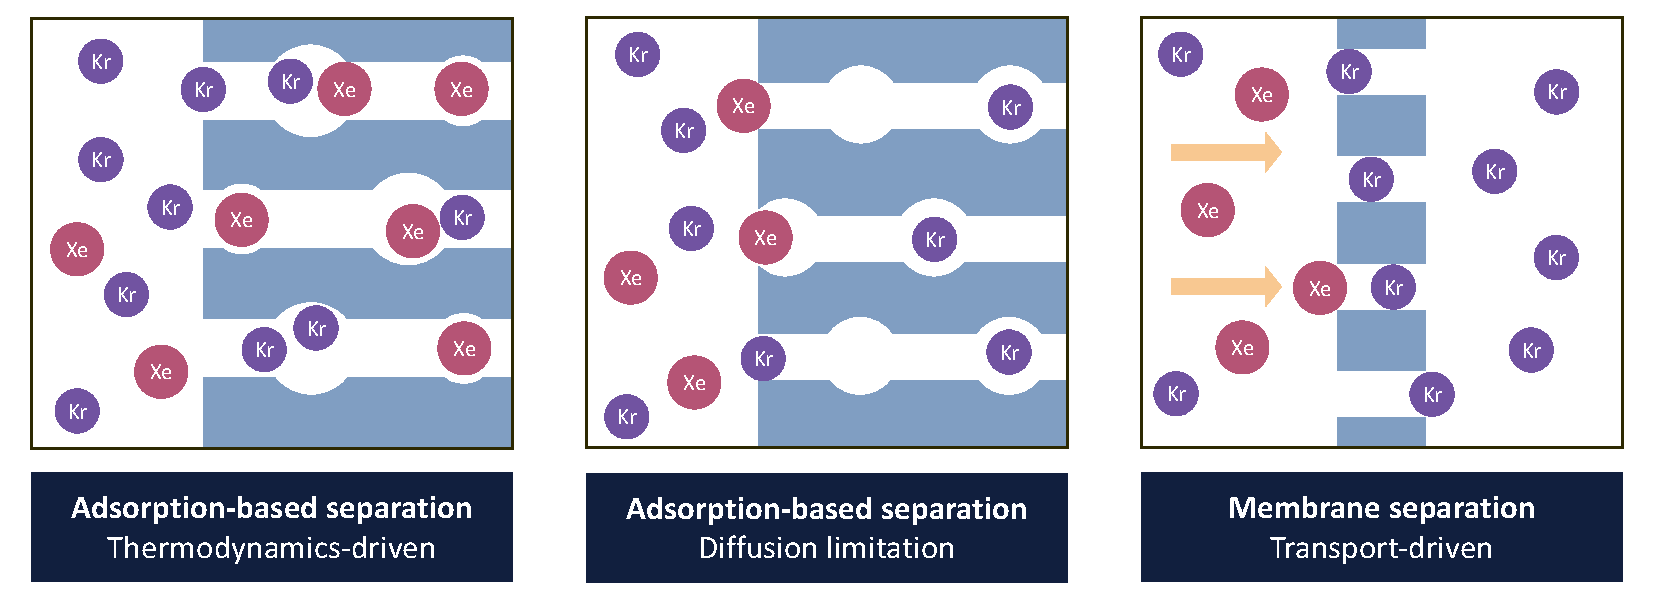
\includegraphics[width=0.95\textwidth]{figures/5-diffusion/Diffusion.pdf}
    \caption{Illustration of the comparative role of the thermodynamic and transport properties for Xe/Kr separation in nanoporous materials. From the transport dominated process of membrane separation to the thermodynamically equilibrated separation processes in the nanopores, different more nuanced cases could emerge where the diffusion imposes kinetic limitations.}
    \label{fgr:intro_diffusion}
\end{figure}

\section{Modeling the Diffusion Process}

% From the macroscopic brownian motion modeled by the
% Fick's law
Since the pollen motion observations of the botannist Brown in 1826, scientists have observed and studied the seemingly erratic movement of particles in a static bulk medium. Later, Fick proposed a macroscopic model of this so-called brownian motion by introduced the coefficient $D$ of a diffusion equation~\ref{eq:fick} (1D) based on experimental measures of the concentration $\phi$.\autocite{Fick_1855} According to this law (valid only for independent particles), at the macroscopic level, the particles tend to move from the most concentrated area of the bulk to the less concentrated one. 

\begin{equation}\label{eq:fick}
  \frac{\partial \phi}{\partial t} = D_x \frac{\partial^2 \phi}{{\partial x}^2}
\end{equation}

To better understand the brownian motion of suspended particles on a liquid Einstein derived a microscopic model of the diffusion motion based on the molecular-kinetic theory of heat on the miraculous year of 1905.\autocite{einstein1905motion} To determine the so-called self-diffusion coefficient (in the following development I will use ``diffusion coefficient'' for short), he followed the motion of a particle assumed independent from other particles and time steps large enough to consider mutually independent two consecutive motions. By using the particle distribution of $N$ independent diffusing particle, he redefined the diffusion coefficient as a function of the mean squared displacement (MSD) of a particle. In a tridimensional space, we have the following Einstein relation:
\begin{equation}\label{eq:einstein}
  \langle {r(t)}^2 \rangle = 2dD\e{diff}t = 6D\e{diff}t
\end{equation}
where  $d$ is the dimension of the space in which the particle diffuses ($d=3$ in a volume) and $r(t)$ is the displacement of a particle from the time $0$ to $t$. The brackets represent the average over all independent trajectories (different particles and different time origins). This equation can be generalized to the diffusion of an adsorbate in the adsorbed phase, which describes how easy it is for a particle to move inside a nanoporous material. A low diffusion coefficient means a limited access to the pores of the structure as illustrated on the Figure~\ref{fgr:intro_diffusion}.

Using molecular simulations of the adsorbate displacements, I will try to model the diffusion coefficient of xenon and krypton inside a nanoporous material. Although other approaches like the Green-Kubo equation exist the relatively less complex Einstein law is prefered for self-diffusion calculations, as shown by the following comparative study~\cite{Maginn_2020}. In this section, I will focus on the different simulation techniques that can be used to evaluate the diffusion in high-throughput screenings. I will try to present different ways of accessing the MSD of a diffusing particles, by beginning from the most straight-forward molecular dynamics to faster methodologies more suitable in screenings such as machine learned surrogate models and kinetic monte carlo simulations.


\subsection{Molecular dynamics}

Molecular dynamics are used to simulate the motion of molecules in a given system. It is usually used to calculate thermodynamic averagings by using an hypothesis on the equivalence between the time averaging and ensemble averaging (ergodic hypothesis); in other system configurations, we can determine mechanical properties, thermodynamic properties or chemical properties. But here, I am more interested in the calculation of diffusion coefficients of monoatomic molecules, and the discussion will be driven toward averaging trajectories to obtain MSD values.

\subsubsection{Simulation details}

Molecular dynamics (MD) aims at describing the motion of particles subjected to the forces of the surrounding particles. It can therefore be seen as a complex integration of the Newton's law of motion. A particle $i$ of position $\mathbf{r}_i$ and mass $m_i$ subjected to a force $\mathbf{F}_i$ resulting of the cumulated interactions with its surrounding is accelerated according to this equation:
\begin{equation}\label{eq:newton}
  m_i\frac{\dd^2 \mathbf{r}_i}{{\dd t}^2} = \mathbf{F}_i
\end{equation}

In a classical modeling, the forces are determined using the well-named forcefield that was previously introduced in the chapter 2. Back there, I only considered intermolecular interactions simply modeled by the Lennard-Jones (LJ) interaction potential between atom pairs, which is also what I will use in this section (of course, it is not the only way of defining a forcefield but just a simplification). Using the LJ potentials $U\ex{LJ}$ (defined in equation~\ref{eq:LJ}), we can derive a vectorial force $\mathbf{f}_{ij}$ between two atoms $i$ and $j$.
\begin{equation}
  \mathbf{f}_{ij} = - \left.{\dfrac{\dd U\ex{LJ}_{ij}}{\dd r}}\right\rvert_{r=r_{ij}} \frac{\mathbf{r}_{ij}}{r_{ij}} = 24\epsilon_{ij}  \left(2{\left(\dfrac{\sigma_{ij}}{r_{ij}}\right)}^{12} - {\left(\dfrac{\sigma_{ij}}{r_{ij}}\right)}^{6}\right) \frac{\mathbf{r}_{ij}}{r_{ij}^2}
\end{equation}
where $\epsilon_{ij}$ and $\sigma_{ij}$ are the LJ parameters of the pair of atoms $ij$. And the resulting force is simply the sum of the forces $\mathbf{F}_i=\sum_{j}\mathbf{f}_{ij}$ exerted by the surrounding atoms $j$. To reduce the computation time required, molecular simulations only consider the atoms within a given cutoff radius. 

Now that we defined the force $\mathbf{F}_i$, we can put a molecule in motion by integrating the equation~\ref{eq:newton} from a time $t$ to a time $t+\delta t$. There are different methods to integrate equation of motion such as the Euler or velocity-Verlet scheme presented in the book of Frenkel et al.\autocite{frenkel2001md} Here, I will focus on the \emph{leap frop} integration implemented in the RASPA2\autocite{dubbeldam2016} software that I used for our simulations. The position $\mathbf{r}_i$ and the velocity $\dot{\mathbf{r}}_i$ are between each time step $\delta t$ using the following equations:
\begin{equation}\label{eq:frogleap_integration}
  \begin{split}
    \dot{\mathbf{r}}_i\left(t+\tfrac{1}{2}\delta t\right) & = \dot{\mathbf{r}}_i\left(t-\tfrac{1}{2}\delta t\right) + \tfrac{1}{m_i}\mathbf{f}_i \\
    \mathbf{r}_i\left(t+\delta t\right) & = \mathbf{r}_i\left(t\right) + \dot{\mathbf{r}}_i\left(t+\tfrac{1}{2}\delta t\right)\delta t
  \end{split}
\end{equation}
From the initial conditions $(\mathbf{r}_i(0),\dot{\mathbf{r}}_i(0.5\delta t))$, we can translate the center of mass of the molecule $i$ to any position $\mathbf{r}_i(t_n=n*\delta t)$. I will skip the rotation step required for polyatomic molecules since the study is restricted to the monoatomic noble gas. The different positions ${\left\{\left(t_n,\mathbf{r}_i(t_n)\right)\right\}}_{n=0,\ldots,N\e{tot}}$ constitute the total trajectory of the MD simulation (to simplify I do not mention the velocities). It is possible to use this total trajectory to derive an average of MSD that could be analysed to calculate the diffusion coefficient.

\subsubsection{Diffusivity calculation using an MD trajectory}

I used the MSD sampling technique implemented in RASPA2\autocite{dubbeldam2016} that was presented in an article~\cite{Dubbeldam_2009} by a few authors of the adsorption simulation software. The approach is based on a modified approach of the order-$\mathbf{n}$ algorithm described in the book~\cite{frenkel2001msd} of Frenkel and Smit. Therefore, I will focus on the so-called multiple-window algorithm used to calculate the diffusion coefficients of xenon and krypton in this chapter. 

To understand it, I will start by explaining what a window algorithm would do and how it generalizes to the multiple-window algorithm.
First, let us consider a single MD trajectory of duration $t\e{tot}=N\e{tot}\delta t$. This trajectory can be used to generate displacement of any size $\tau$. Naively, we can start by taking ${\lVert\mathbf{r}_i(\tau)-\mathbf{r}_i(0)\rVert}^2$ as a square displacement of a sub-trajectory $\mathcal{T}(0\rightarrow\tau)$ of duration $\tau$. 
However, it is not enough to make a statistically meaningful average of the MSD as described in the Einstein equation\ref{eq:einstein}. Using the hypothesis of independence between two movements of the same particle separated by a time $\delta t$ used in Einstein's paper~\cite{einstein1905motion}, a shift of the origin of time by $\delta t$ would generate another trajectory. We can repeat this process $i$ times while $\tau + i\delta t\leq t\e{tot}$. This would be very accurate, but also very inefficient in the case where $\tau \gg \delta t$ since two consecutive sub-trajectories $\mathcal{T}(i\delta t\rightarrow\tau+i\delta t)$ and $\mathcal{T}((i+1)\delta t\rightarrow\tau+(i+1)\delta t)$ would be very similar. 

To efficiently sample the trajectory into sub-trajectories that are independent we can use a sampling time step of $\delta \tau\lesssim\tau$ chosen to be in the same order of magnitude as $\tau$. To do so, the window approach would first define a value $\delta \tau$ and generate $N_{\tau} = \lfloor(t\e{t ot} -\tau)/ \delta\tau \rfloor$ different sub-trajectories $\left\{\mathcal{T}(0\rightarrow\tau), \mathcal{T}(\delta\tau\rightarrow\tau + \delta\tau), \ldots, \mathcal{T}(N_{\tau}\delta\tau\rightarrow\tau + N_{\tau}\delta\tau)\right\}$ of duration $\tau=k\delta\tau$, where $k$ is an integer between $1$ and $K$ that defines the time window we want to sample. By doing so, we get the MSD $\langle {r(\tau)}^2 \rangle$ for duration values $\tau$ equal to $\delta\tau, \ldots, K\delta\tau$. The relation $\langle {r(\tau)}^2 \rangle$ can then be fitted to the equation~\ref{eq:einstein} to obtain the diffusion coefficient if the relation is linear. The trajectory generation of the window approach is illustrated on the Figure~\ref{fgr:window_msd} for a decomposition into sub-trajectories of a duration $\tau=3\delta\tau$ shifted by $\delta\tau$.

\begin{figure}[ht]
  \centering
    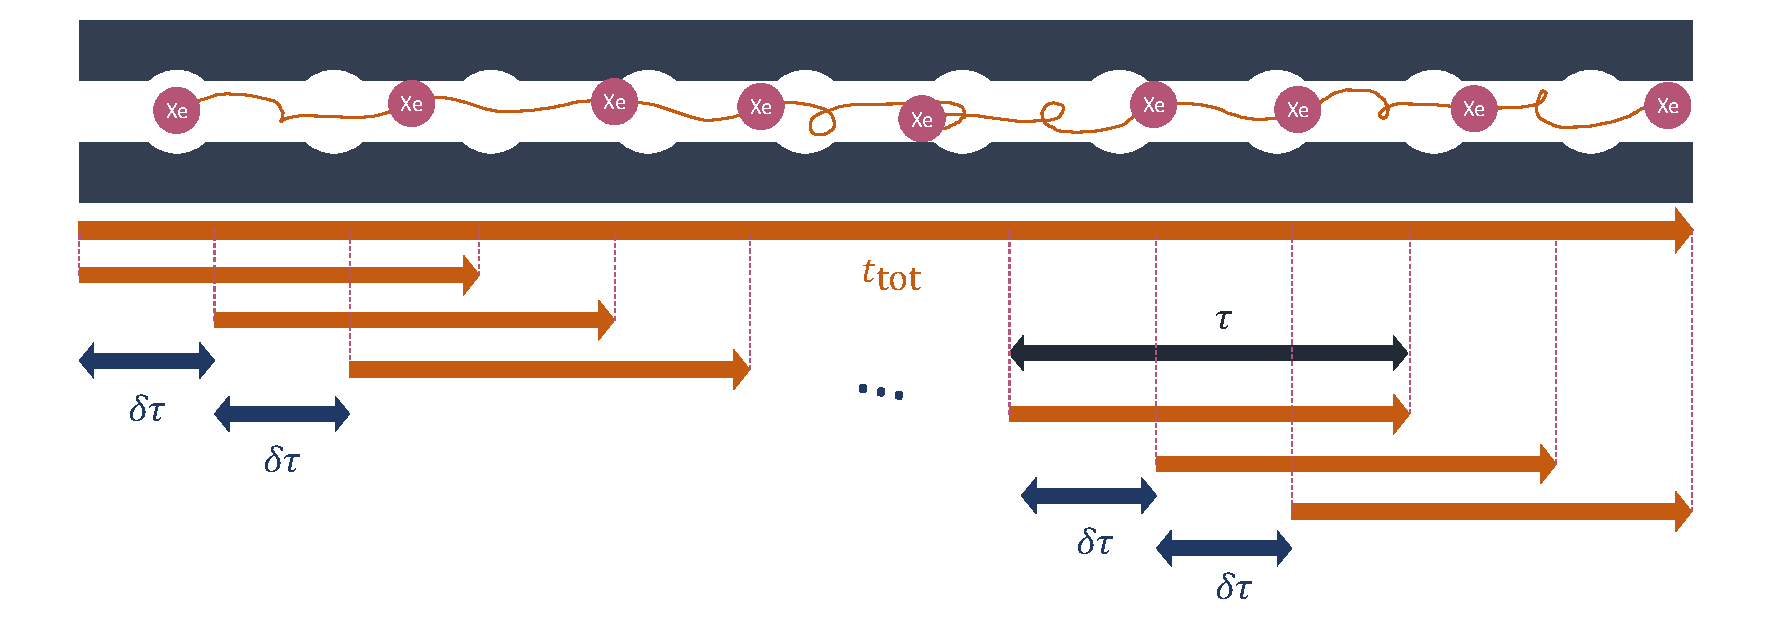
\includegraphics[width=0.95\textwidth]{figures/5-diffusion/diffusion_averaging.pdf}
    \caption{Illustration of the generation of trajectories of size $\tau$ by shifting the origins of multiple durations $\delta\tau$. }\label{fgr:window_msd}
\end{figure}

The major drawback of this method is that we need to define a timescale $\left\{\delta\tau, \ldots, K\delta\tau\right\}$ beforehand. In order to be able to access the different timescales in a single simulation, we can perform a multiple-window algorithm developed by Dubbeldam et al.\ and used in the RASPA2 software to compute mean squared displacements (MSD) in a molecular dynamics simulation.

The different time windows are defined in a recursive way using the default parameters of RASPA2. The first time window is defined by $K=25$ displacements of duration $\delta t, 2\delta t, \ldots,(K-1)\delta t$ with a shift of $\delta t$ (the default shift value $\delta t$ of the first window can be changed with the parameter SampleMSDEvery). The second window is now based on a sampling time $\delta \tau_1 = K\delta t$ and the sub-trajectories will have durations of $\left(\tau_1^{(1)} = \delta\tau_1\right),\ldots,\left(\tau_1^{(K-1)} = (K-1)\delta\tau_1\right)$. We, then, repeat the process recursively, and the $i$\e{th} window would have a sampling time of $\delta \tau_i = K^i\delta t$ and sub-trajectories durations of $\left(\tau_i^{(1)} = \delta\tau_i\right),\ldots,\left(\tau_i^{(K-1)} = (K-1)\delta\tau_i\right)$, for each of them a window algorithm similar to the one described above is applied. The algorithm stops when no window can be generated anymore, when $\tau_n^{(k)}>t\e{tot}$ with $n$ being the index of the window and $k$ the index in the single-window algorithm that defines the time we want to sample with regard to a sampling time $\delta\tau_i$. The time-scale $\delta \tau_i = K^i\delta t$ we sample follows a geometrical progression and very different time-scales can be accessed using this method in order to find the time-scale corresponding to the diffusion regime (linear relation between the MSD and the duration of the sub-trajectories used in the averaging). For example on the Figure~\ref{fgr:MSD_init}, we can see the different timescales and the exponent value $b$ of a fit to a function of type $x \mapsto ax^b$ for the different time windows --- values of $b$ near $1$ can be associated to a diffusion regime. The determination of the diffusion coefficient is now reduced to a simple fitting problem that will be explained in more details in the presentation of the diffusion coefficient screening in section~\ref{sct:md_screening}.

This methodology can then be used replicated to thousands of structures to characterize the diffusion properties of these materials. Several screenings have already been carried out in the literature as presented in the chapter 1 in the section dedicated to transport property screenings. I will now dive a little deeper in the prediction of these quantities using machine learning.

\subsubsection{ML modeling}

In a very recent study, Daglar et al.\ used an ML model to predict the diffusion coefficient of a 100 thousand hypothetical MOFs using the data for about 5000 CoRE MOF structures.\autocite{Daglar_2022} Along with very standard geometrical descriptors, they used chemical composition descriptors and the heat of adsorption as the input features of their machine learning model to predict the diffusion coefficients of \ce{H2}, \ce{CH4}, \ce{N2} and \ce{He} in the different MOF materials of CoRE MOF 2019 (training) and of hMOF (testing). The combination of kinetic data with thermodynamic data for the characterization of MOf materials is a very interesting approach. However, the major drawback of most of the approaches in the literature is the lack of structure--property relationship to understand the microscopic origins of the diffusion coefficient values.

Simarly to what I have done on the thermodynamic screening (chapter 2--4), in our approach to tranport property screening, I will also start by drawing structure--property relationships between the diffusion coefficient and the geometrical descriptors of the MOF structures. And in an attempt to have a deeper understanding of the diffusion process, I will try to evaluate the diffusion activation energy using energy grid-based methods described in the literature. All these techniques aim at better predicting the diffusion coefficients either in a direct calculation or in an ML surrogate model. To achieve that, I will start by introducing the kinetic Monte Carlo approach that is less accurate than the MD approach but is indeed much more efficient.

\subsection{Lattice kinetic Monte Carlo}

The lattice kinetic Monte Carlo method relies on a pre-defined lattice of stable points corresponding to adsorption sites. Each site connected to another if there is a diffusion path (narrow channel) that connects them. To calculate the probability of transition from one site to another, I need to define a transition state (TS) in the narraow channel which correspond to the highest energy point on the minimal energy diffusion path (the saddle point). The probability of transition would therefore be defined with regard to the energy barrier to overcome in order to cross the channel. Once the lattice defined, we only need to propagate an adsorbate from one site to another using the different transition probabilities, which gives a coarse-grained trajectory compared to the one obtained in a MD simulation, but is perfectly usable to compute the MSD and calculate a diffusion coefficient.


\begin{figure}[ht]
  \centering
    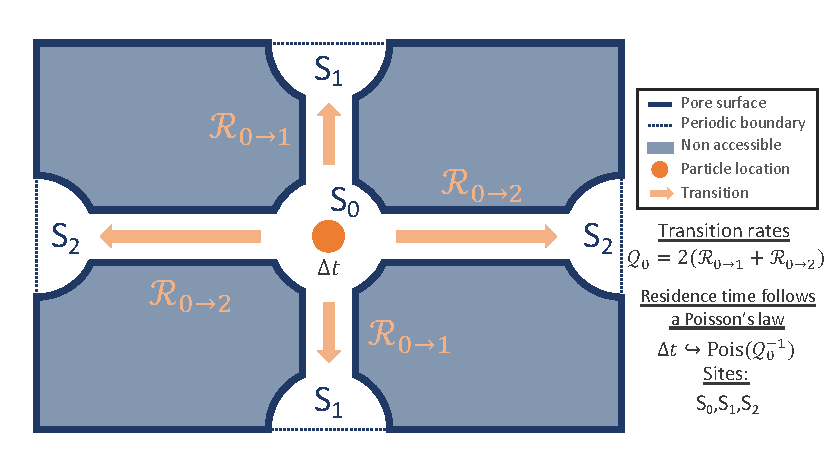
\includegraphics[width=0.9\textwidth]{figures/5-diffusion/kinetic_MC.pdf}
    \caption{Illustration of the core principle of lattice kinetic Monte Carlo in a periodic system. The particle moves inside the periodic system according to the transition probabilities to move from one site to another. The transition rates are determined using the activation energy needed to move to the transition state between the two stable adsorption sites as shown in equations~\ref{eq:trans_rate_path} and~\ref{eq:trans_rate}. }\label{fgr:kMC_principle}
\end{figure}

\subsubsection{Transition state theory for diffusion}

The transition state theory is usually used in chemistry to explain the kinetics of a reaction. To do so it compares the energy of the reactants before reacting and the one of the transition state to calculate the rate of the reaction. This reaction rate along a reaction path is proportional to the ratio of the Boltzmann factor at the transition state and the integration of the Boltzmann factors along the reaction path.

This definition can be directly transposed to the case of a diffusion path instead of a reaction path, and we can define the diffusion rate $\mathcal{R}_{0\rightarrow 1}$ from site $0$ to $1$ as follows:
\begin{equation}\label{eq:trans_rate_path}
  \mathcal{R}_{0\rightarrow 1} = \kappa\sqrt{\frac{k\e{B}T}{2\pi m}}\frac{e^{-\beta E(\mathbf{r}\ex{TS})/k\e{B}T}}{\int\e{path}e^{-\beta E(\mathbf{r})/k\e{B}T}\dd\mathbf{r}}
\end{equation}
where $\kappa$ is the Bennet-Chandler dynamic correction factor,\autocite{BENNETT1977} and  $\kappa=\tfrac{1}{2}$ if it is equiprobable to reach both sites from the transition state. This approach calls for the determination of the optimal diffusion path before carrying out the determination fo the diffusion rate. This is for instance the approach adopted by Wang et al.\ in their screening for noble gas separation, where they determined the minimal energy path before calculating diffusion rates.\autocite{Wang_2022}

Another approach is to determine a surface of transition through which the adsorbate would pass to diffuse along the channel of the material. This approach calls for the determination of the surface of transition only, but it relies on another definition of the transition rate $\mathcal{R}_{0\rightarrow 1}$:
\begin{equation}\label{eq:trans_rate}
  \mathcal{R}_{0\rightarrow 1} = \kappa\sqrt{\frac{k\e{B}T}{2\pi m}}\frac{\int_{\mathcal{S}(TS)}e^{-\beta E(\mathbf{r})/k\e{B}T}\dd\mathbf{r}}{\int_{\mathcal{V}(\text{S}_0)}e^{-\beta E(\mathbf{r})/k\e{B}T}\dd\mathbf{r}}
\end{equation}
where the integration for the transition state is done on a bottle-neck surface that a diffusing particle need to cross in order to go from the volume occupied by a site $0$ to the one occupied by $1$.

\subsubsection{TuTraST algorithm for kinetic MC}\label{sct:tutrast}

In this section, I will focus on the second approach that relies on the determination of a transition state as a surface. This approach has been developed by Mace et al.\autocite{Mace_2019}\ and relies on detecting the merging points between basins representing the adsorption pores. The algorithm developed is called TuTraST, which stand for Tunnels and Transition States. It is a search algorithm that aims at finding the tunnels and the transition states that separate different adsorption ``basins'' within them. Once the adsorption sites, the transition states and the tunnels that connect them are found, we can calculate the hopping rates between the stable adsorption sites using the equation~\ref{eq:trans_rate}. Finally, a lattice kinetic Monte Carlo simulation can be used to move particles within simplified hopping diffusion system to determine the MSD and eventually the diffusion coefficient. 

\begin{figure}[ht]
  \centering
    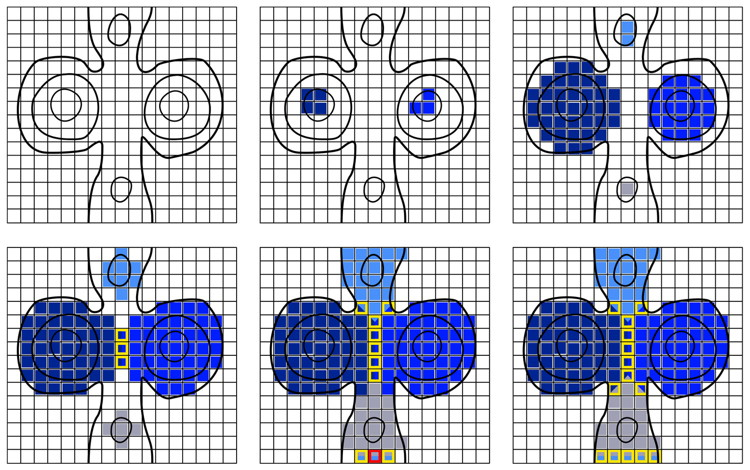
\includegraphics[width=0.6\textwidth]{figures/5-diffusion/tutrast.jpg}
    \caption{ Illustration of the cluster growth and the identification of boundary points in the TuTraST algorithm\autocite{Mace_2019}. the clusters are grown from left to right and top to bottom. A tunnel is detected when the points are connected all the way from one periodic boundary to another (red). The boundary points assigned to the TS surface are indicated in yellow. Reprinted with permission from the original paper~\cite{Mace_2019} copyright \copyright\ 2019 American Chemical Society. }\label{fgr:tutrast}
\end{figure}

In practice, we need to calculate an energy grid that will be used to detect all the different components of lattice. The algorithm iterates over different energy values from $E\e{min}+\delta E, \ldots, E\e{min}+N\delta E$ so that the maximum energy is below an energy cutoff we fixed at the start $E\e{min}+N\delta E<E\e{cutoff}$. At the inital step, the clusters of grid points with an energy below $E\e{min}+\delta E$ are formed naturally depending on whether they are connected or not. Then, at an iteration level $L$, the previous clusters found at iteration $L-1$ are grown layer by layer (one layer corresponds to the immediate neighbors on the grid), as shown on the Figure~\ref{fgr:tutrast}. If the layer touches another cluster, then a boundary point is identified --- it is only accepted if the energy difference between minimum energy of the two touching basins and the boundary point value is high enough, else the barrier is negligible and the basins are merged. At the end, the boundary values will be clustered and assigned as the transition surface between different pairs of adsorption basins. If the points of basins and bboundary surfaces are connected all through, then we can define a tunnel in which diffusion can occur. Finally, when we iterated enough steps, and tunnels with different basins separated by transition state surfaces are defined. We can now run a kinetic Monte Carlo to determine the diffusion coefficient within each tunnel. The diffusion coefficient in the material will correspond to a weighted average of the diffusion coefficient in each tunnel, the weight simply corresponds to the probability of presence in each tunnel, which corresponds to the sum of the Boltzmann factors (proportional to the Henry coefficient in a given tunnel). 

This approach is very promising since it is much more efficient than the MD simulation based techniques. With an implementation in Matlab (not very computationally efficient), the code is already out-performing most of the MD simulations for diffsuion coefficient calculation, with a minimal cost in accuracy as shown in their screening of diffusion coefficients in zeolites. By using the C++ programming language, I tried to rewrite the algorithm for a more efficient search of the transition states. At this point of the development, I stopped at the determination of the diffusion activation energy which is independent of the detection of the transition state. And, in section~\ref{sct:algo_diff}, I will give the algorithmic detail for the determination of the diffusion activation energy in nanoporous mateirals using our in-house algorithm as well as the projected development to achieve a faster lattice kinetic Monte Carlo simulation inspired by the TuTraST algorithm.


\section{Self-diffusion screening}\label{sct:md_screening}

To complete the thermodynamic screenings that I performed in the chapters 2--4, I also carried out a transport property screening. In this section, I will provide a description of the screening approach as well as the analysis of the diffusion coefficients compared with typical geometrical descriptors.

\subsection{Diffusion in a selective material}

Before going into the details of the screening study, I will present the approach adopted for the diffusion coefficient calculation using MSD values, on one example, SBMOF-1\autocite{Banerjee_2016}. This preliminary study will help us calibrate the time parameters (time step, maximum time) that will be used in the final screening study.

First, I ran a molecular dynamics simulation of 500 million steps (about 1--2 days of simulation) with a thousand initialization steps and 100 thousand equilibration steps to model a xenon diffusing in the KAXQIL\autocite{Banerjee2012} MOF at infinite dilution. To be at infinite dilution, I set the box size so that no interactions occur between the different adsorbates. And as shown on the Figure~\ref{fgr:MSD_init}, there are different time-scales at which different transport phenomena occur. 

From \SI{1}{\fs} to \SI{1}{\ps}, there is a ballistic regime with a squared dependence of the mean squared displacement. For a particle of mass $m$, the MSD $\langle {r(\tau)}^2 \rangle$ in this regime follows a simple ballistic relation (length equals velocity multiplied by time):
\begin{equation}
  \langle {r(\tau)}^2 \rangle = v_m^2 \tau^2 = \frac{k\e{B}T}{2\pi m}\tau^2
\end{equation}
where $v_m$ is the average velocity of a particle that follows the Maxwell-Boltzmann distribution at temperature $T$. If we calculate the squared mean velocity $v_m^2$ using the standard Maxwell-Boltzmann relation, we get a value of \SI{3}{\square\m\per\square\second}, which is very close to the value of \SI{2.8}{\square\m\per\square\second} obtained by the fit shown right plot of Figure~\ref{fgr:MSD_init}. This first regime simply corresponds to the movement of the particles subjected to the thermal agitation and is of little interest for diffusion. 

\begin{figure}[ht]
  \centering
    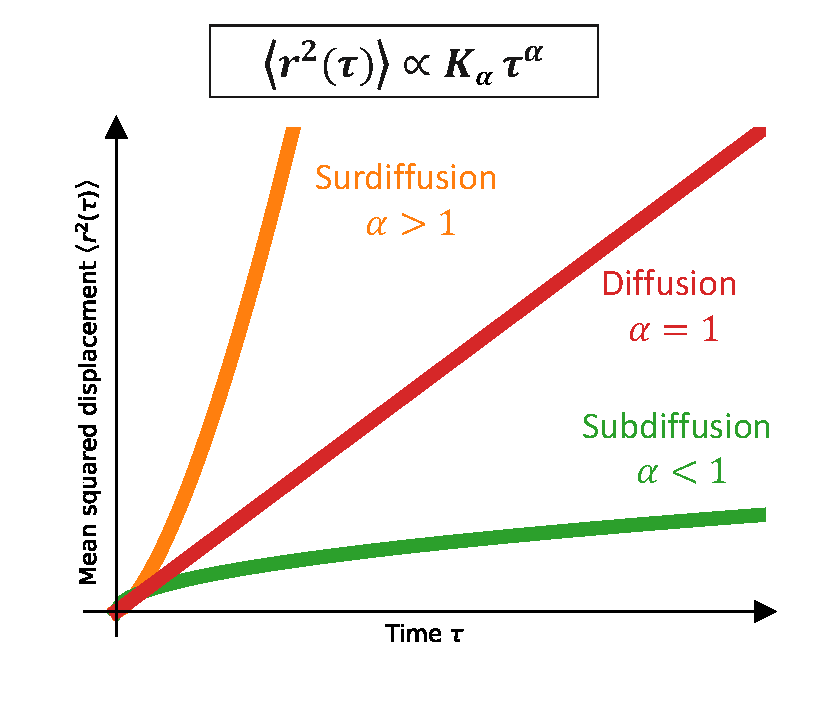
\includegraphics[width=0.48\textwidth]{figures/5-diffusion/MSD_anomalous_diffusion.pdf}
    \includegraphics[width=0.48\textwidth]{figures/5-diffusion/MSD_Xe_KAXQIL_clean.pdf}
    \caption{Left: Different regimes that could be observed in an MSD plot as a function of time. The ballistic regime can be considered superdiffusional, the normal diffusion is simply a linear relation as described in the Einstein equation\ref{eq:einstein}, and the subdiffusion regime often occurs in obstructed media like nanoporous materials. The different regimes can be found on the right plot of an actual MSD calculated using the multiple-window method. The fittings are done using a generic function $K_\alpha\tau^\alpha$ and the exponents $\alpha$ are given in the legend. }\label{fgr:MSD_init}
\end{figure}

Then, there is a transition from the ballistic regime to the pseudo-diffusional regime (the exponent does not reach $1$ yet) that we observe in cyan on the plot. Between \SI{1}{\ps} and \SI{100}{\ps}, there is a so-called subdiffusion regime, where the MSD has a power function of the time $\langle {r(\tau)}^2 \rangle=K_\alpha\tau^\alpha$ with an exponent inferior to $1$ as illustrated on the left plot of Figure~\ref{fgr:MSD_init}. This regime corresponds to the confinement of the xenon particle inside an adsorption pore, there is only thermal vibration occuring and no diffusion hopping is observed at this time-scale. And diffusion seems to start occuring at the \SI{10}{\ns} time-scale. As shown on the Figure~\ref{fgr:MSD_linear_init}, the MSD between \SI{0.01}{\ns} and \SI{0.4}{\ns} really represents a sub-diffusional regime due to the confinement imposed by the nanopores of KAXQIL, but at \SI{0.4}{\ns}--\SI{9}{\ns}, the MSD start to have an exponent closer to $1$ and a linear fit is possible although not perfect. Ideally, we would want to sample trajectories in the order of tens of nanoseconds, which is the next time-scale. But with an MD time step of \SI{1}{\fs}, this would mean multiplying the computation time by at least 5 (1--2 weeks for one MD simulation), which begins to be prohibitive. 

\begin{figure}[ht]
  \centering
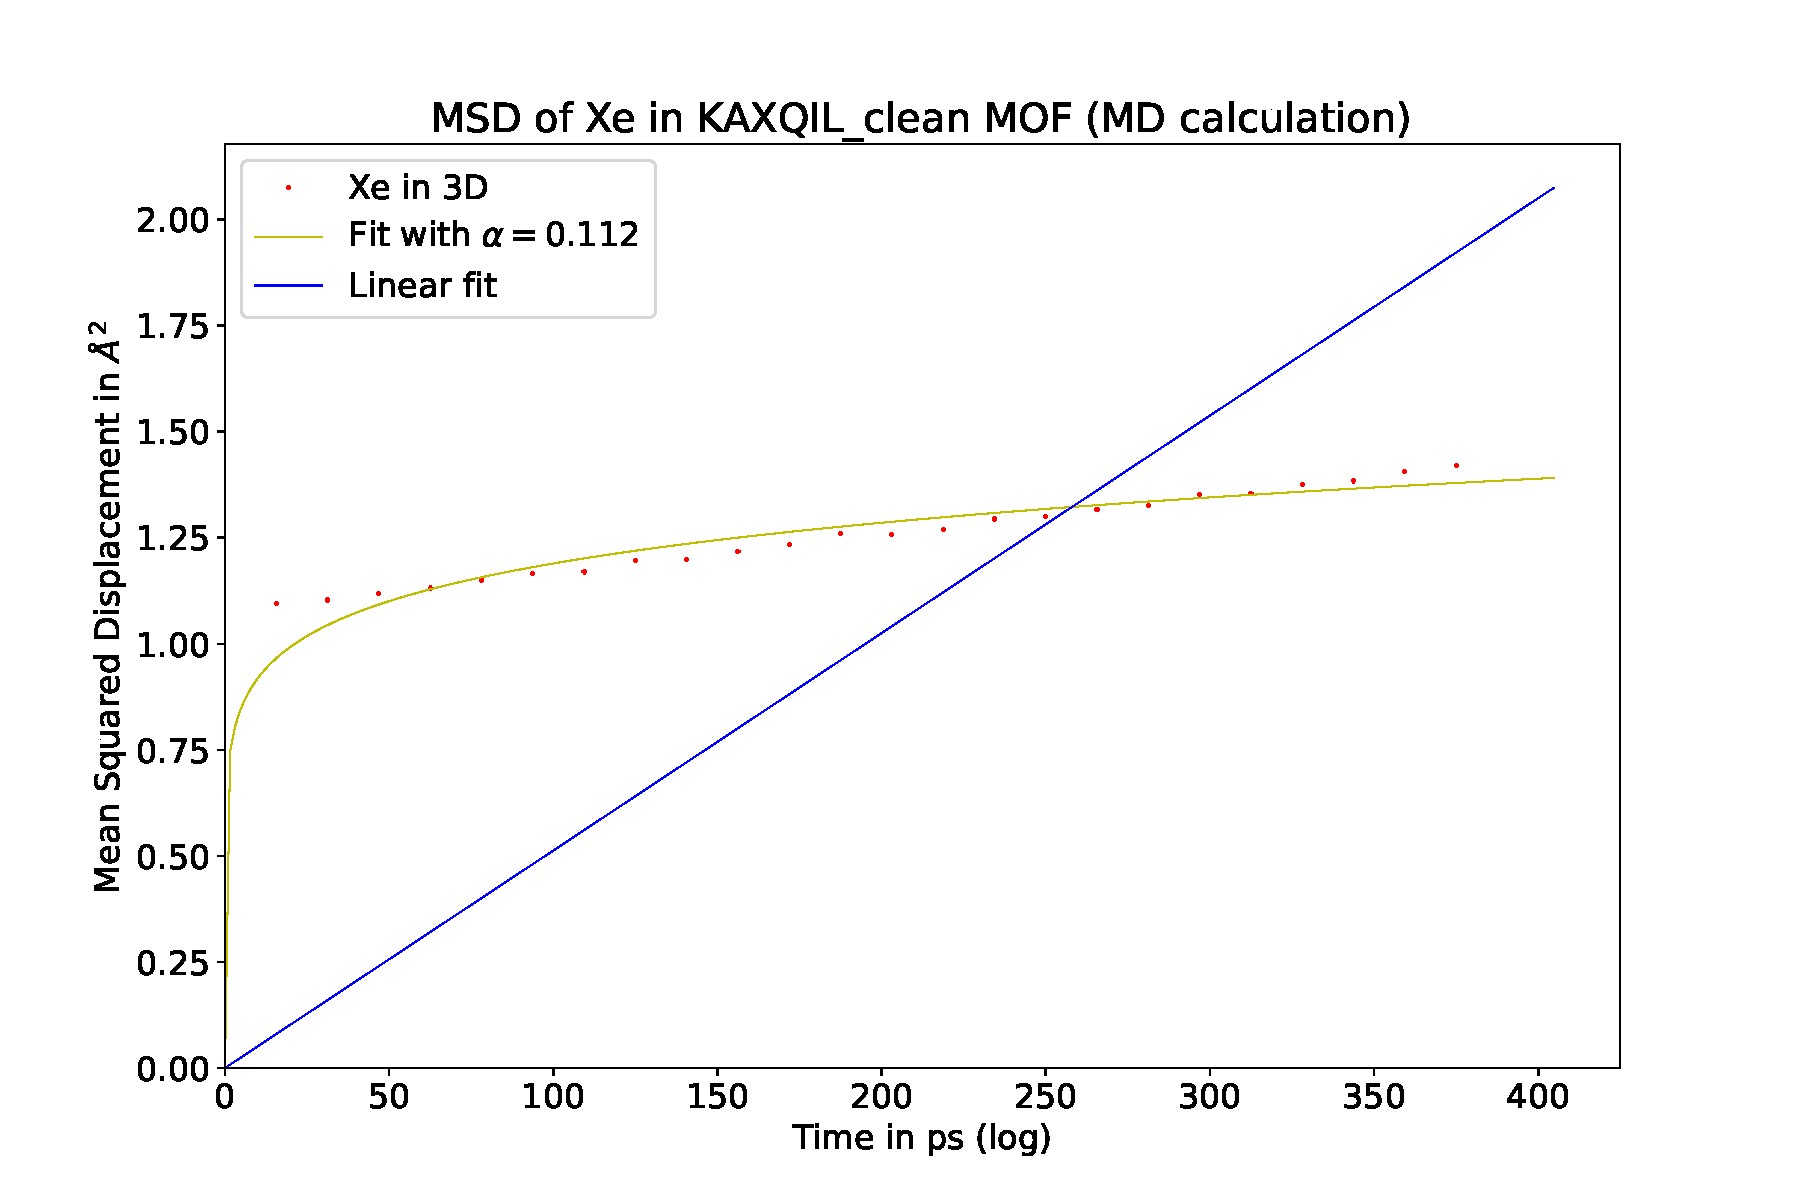
\includegraphics[width=0.48\textwidth]{figures/5-diffusion/MSD_Xe_coeff_KAXQIL_clean_1.pdf}
\includegraphics[width=0.48\textwidth]{figures/5-diffusion/MSD_Xe_coeff_KAXQIL_clean_2.pdf}
\caption{ Plots of the MSD at the last two time-scales considered on the Figure~\ref{fgr:MSD_init}. On the left, the time-scale between \SI{0.01}{\ns} and \SI{0.4}{\ns} is considered, the MSD is fitted by a power function with the same exponent as one determined earlier, and a linear fit is given to show the incompatibility with the diffusion equation. On the right, we have the same approach but for the time-scale between \SI{0.4}{\ns} and \SI{9}{\ns}. }\label{fgr:MSD_linear_init}
\end{figure}

If we use the right plot of Figure~\ref{fgr:MSD_linear_init} to fit a linear relation and deduct the diffusion coefficient, we can have an underestimated value of the diffusion coefficient of $2.24\times 10^{-8}$~\si{\square\cm\per\s} --- it is an underestimation because the MSD is rather concave, which reduces the slope in the fitting process. This value is already a good estimation of the diffusion coefficient considering the rather high exponent $\alpha$ value in the with regard to $K_\alpha\tau^\alpha$.

Since there is an element of randomness in the initial position of xenon (block pockets have been calculated for a \SI{1.5}{\angstrom}-radius probe), we need to measure the effet of running different MD simulations of the value of the diffusion coefficients. To measure this uncertainty across different MD simulations with different initial positions determined by with different random seed. In RASPA2, the random seed is simply equal to the UNIX time upon launching the MD simulation. This ensures that a different random seed is given to the $10$ different MD simulations we launched using the exact same parameters as mentioned previously. I found that the average diffusion coefficient value equals $2.13\times 10^{-8}$~\si{\square\cm\per\s} and the standard deviation equals $0.37\times 10^{-8}$~\si{\square\cm\per\s}, which represents about {17\%} of the average value. We could estimate the uncertainty to about {17\%} on the diffusion coefficient for a rather low coefficient around $10^{-8}$~\si{\square\cm\per\s}, we could expect lower uncertainty for less obstructing materials. 

Now that I have more confidence on the method, I will try to probe higher time-scales than the one accessible with an MD time step of \SI{1}{\fs}, because the diffusion regime seems to be occuring rather at the \SI{10}{\ns} time-scale. I ran a first calculation with 500 million step to validate the diffusion coefficient value. The time window between \SI{2}{\ns} and \SI{47}{\ns}, and the MSD are calculated from about 200 sampled trajectories, which gives rather correct values. We can obtain a more accurate diffusion coefficient of $2.6\times 10^{-8}$~\si{\square\cm\per\s}, which is very close to the one obtained in the previous approach. The value is slightly higher (which is expected) since the previous values was over-estimated. This approach is therefore consistent with the previous one.

\begin{figure}[ht]
  \centering
  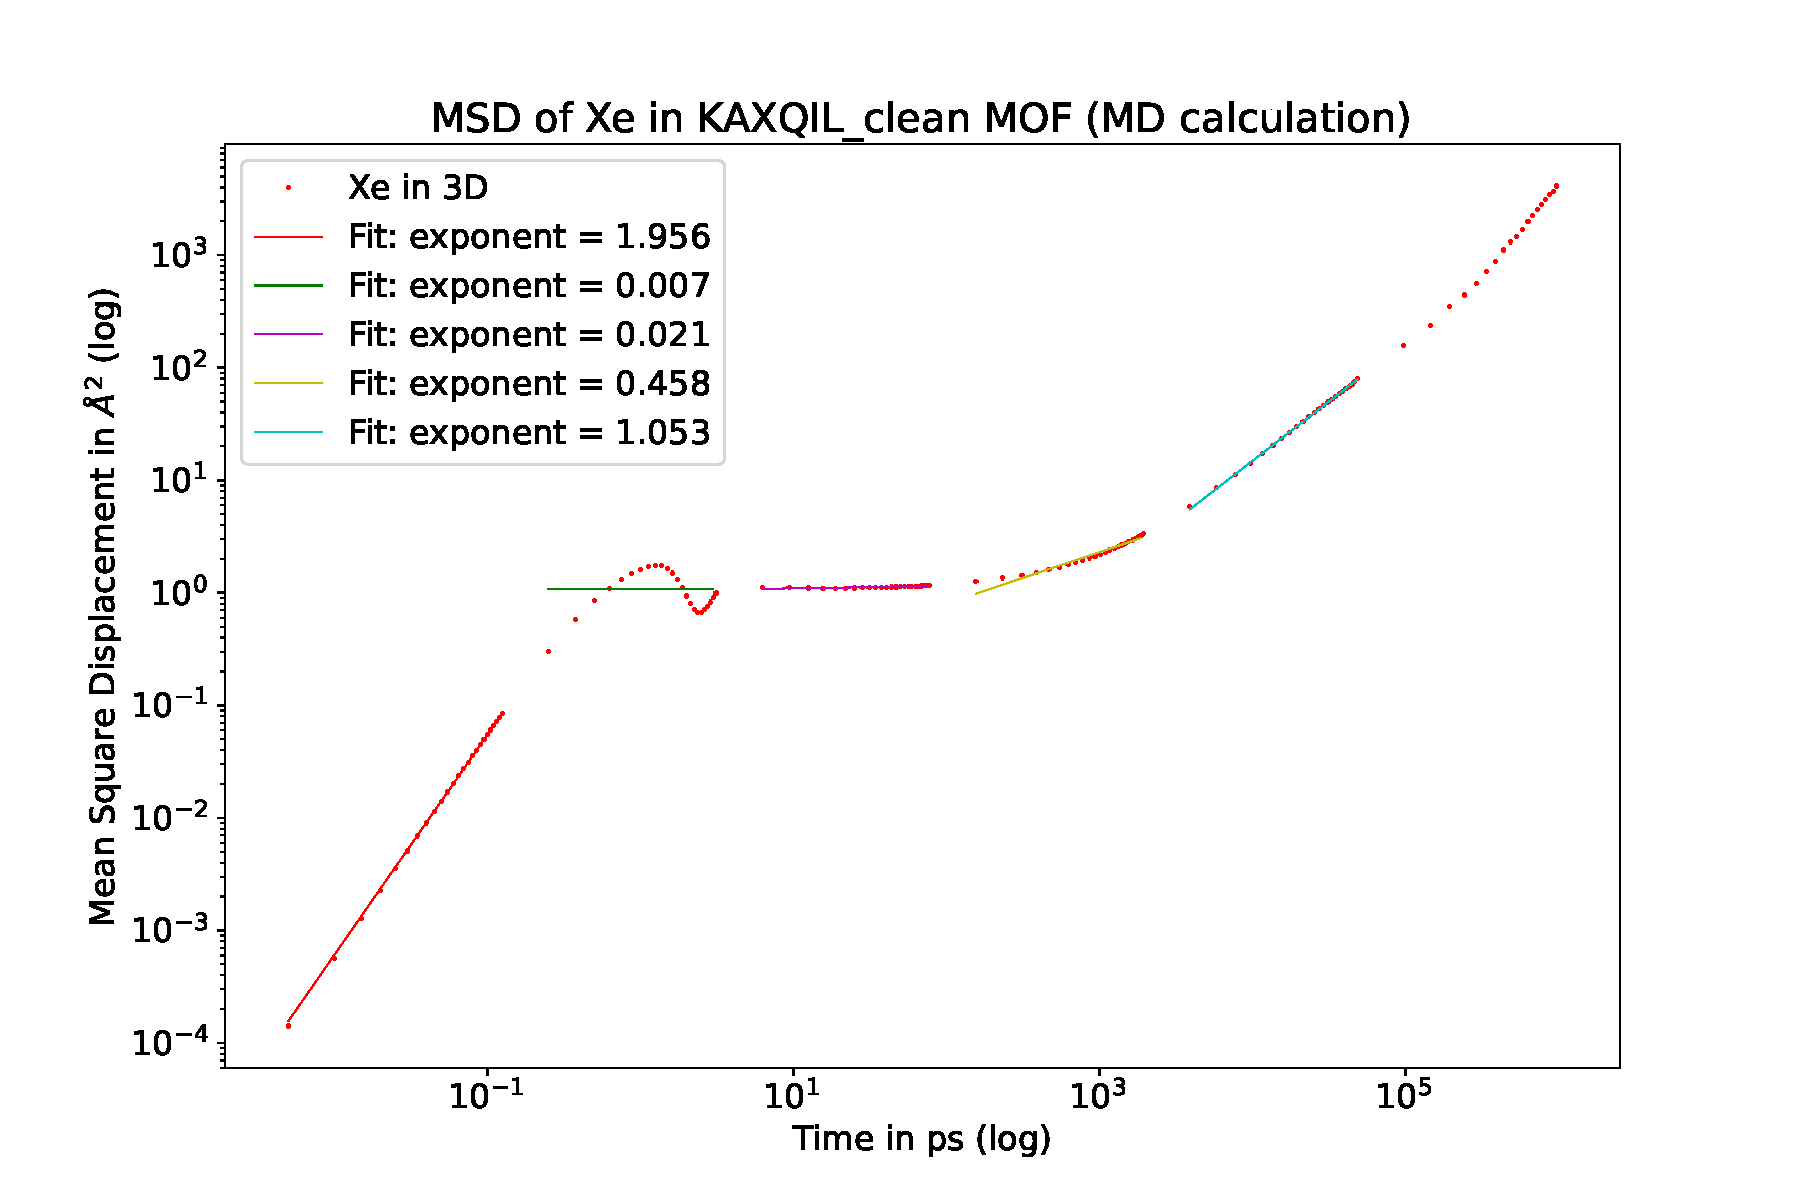
\includegraphics[width=0.48\textwidth]{figures/5-diffusion/MSD_Xe_KAXQIL_clean_5fs.pdf}
  \includegraphics[width=0.48\textwidth]{figures/5-diffusion/MSD_Xe_coeff_KAXQIL_clean_5fs.pdf}
\caption{ On the left, the MSD in log-log scale and a fit to the relation $\text{MSD}(/tau) = K_\alpha\tau^\alpha$ using an MD simulation of a \SI{5}{\fs}-timestep and 500 million steps. I find a better linear fit with this new configuration of the MD simulation than on the Figure~\ref{fgr:MSD_init}, because we explore more time-scales using the same amount of computational resource. On the right, we can find the MSD on time-scale of diffusion regime. The linear fit is better than on the Figure~\ref{fgr:MSD_linear_init}.}\label{fgr:MSD_5fs}
\end{figure}

To further back-up the use of a higher time integration step, we need to understand the origin of the value of \SI{1}{\fs}. This value is usually justified by the Nyquist-Shannon sampling theorem that implies the integration step to be at most half of the period of the fastest vibration within the system. If we take a C--H vibration, the maximum time step value is \SI{5}{\fs}, and to be on the safe side, a time step of $1$--$2$~\si{\fs} is chosen in most of the diffusion studies in nanoporous materials.\autocite{Bukowski_2021} But in our system of a xenon diffusing in a rigid environment, we actually don't have any vibrational limitations as described earlier. I think that the use of higher time steps in this situation can be an easy way to access higher time-scales; however, furhter studies need to be performed to be sure of the validity of the quantities we derive from these MD simulations. The value of \SI{5}{\fs} is on the higher side of what we usually see in MD simulations, but it can be justified by the rigidity of the framework and the adsorbate we consider. Even higher time steps could be tested, but to be sure of the results I chose this reasonable middle ground of \SI{5}{\fs} for all our high-throughput screening of the transport properties.


\subsection{High-throughput screening of diffusion coefficients}

\subsubsection{Screening procedure}

In order to include the transport properties in our analysis, I performed MD calculations of a xenon or krypton at infinite dilution (no guest--guest interactions) for the 6,525 non-disordered most selective materials. For each of them, 500 million steps of MD were planned in the RASPA2 script in the calculation machines and 2 to 3 restarts were done on the slowest simulations so that every MSD data were obtained after 2--3 days. After this process, only 432 structures have finished the planned 500 million steps, but it does not mean that the MSD is not exploitable for the determination of the diffusion coefficients. 

To determine the diffusion coefficients I analyzed two time-scales (2--47\si{\ns} and 50--950~\si{\ns}) to fit the MSD with a linear function. I chose the linear fit with the highest determination coefficient (within $0$ and $1$) of both time-scales to output a value of diffusion coefficient. After this step, I removed structures with a determination coefficient lower than $0.9$ and used the 5,125 remaining structures to draw structure--diffusivity relationships --- these structures for which I have a good degree of confidence on the diffusion coefficient values will be comparatively studied against different geometrical and thermodynamic quantities in this section

This approach only probes the linear relations between the MSD and time to determine the self-diffusion at infinite dilution. I did not analyze the nature of the transport property (e.g. single-file diffusion\autocite{Lin_2005}) by comparing for example the exponent of a generalized formula $\text{MSD}(/tau) = K_\alpha\tau^\alpha$ with structural dscriptors. I did not study the more complex diffusion at higher loading values, which could be more accurately described by a collective diffusion coefficient instead of the self-diffusion coefficient. The goal of this study is to find materials that do not present a kinetic limitation as it is the case for KAXQIL\autocite{Banerjee2012} (xenon has a diffusion coefficient that is about ten thousand times lower in the material than outside).

\subsubsection{Structure--diffusivity relationships}\label{sct:xenon_diff_screen}

In this section, I will present the different relations the diffusion coefficient may or may not have with the geometrical descriptors. I decided to use a forcefield-dependent definition of the radii so that it better correlates with the results of the MD simulation that uses the UFF forcefield. The different geometrical descriptors are then calculated using Zeo++ and these radii to calculate the PLD, the largest sphere diameter D$_{if}$ along a free path, the surface area and the pore volume, as already explained in the chapter 2. To further justify the use of the UFF-based radii, the original paper~\cite{Hung_2021} showed the better correlation of the PLD to the diffusion constant, and we can also see it from the Figure~\ref{fgr:diff_pld}. The PLD calculated by the standard CCDC defined atom radii does not fit the diffusion coefficient as well as the UFF-defined PLD. As shown in a smaller scale in the article~\cite{Haldoupis_2010} (see Figure~\ref{fgr:Haldoupis_2010} in the chapter 1), there is a linear relation between the diffusion activation energy (logarithmic transform of the diffusion coefficient) and the PLD, and this linear relation is much more noisy for the PLD defined by the standard CCDC radii than for the UFF-based PLD.

Beyond the practical considerations on the geometrical descriptor calculations, the PLD explains the outlines of the variation of diffusion performance inside a nanoporous material. First there is a the linear relation previously highlighted, and then there is a sort of noisy plateau. In the first zone, the xenon is constrained by channels narrower than its kinetic radius. The wider the channel the higher the diffusion coefficient is, and this positive correlation persists until the channel is wider than about \SI{4.6}{\angstrom}. After this threshold, the diffusion coefficient is rather stable around $3\times 10^{-4}$~\si{\square\cm\per\s}, and the variations can only be explained by other phenomena such as the tortuosity inside nanopores or chemical nature of the surface of the nanopores. This value of diffusion coefficient can be interpreted as the diffusion coefficient of a ``free'' xenon that is less affected by the surrounding pore surface. The channels are large enough so that the xenon is only a little slowed down, for values of the PLD over \SI{5}{\angstrom}. These results are compatible with experimental data that measured the diffusion coefficient of xenon dissolved in water at different temperature conditions, and found a value of $10^{-5}$~\si{\square\cm\per\s} at \SI{303}{\kelvin},\autocite{Wise1968} which is consistent with values centered around $3\times 10^{-4}$~\si{\square\cm\per\s} at the plateau.

\begin{figure}[ht]
  \centering
    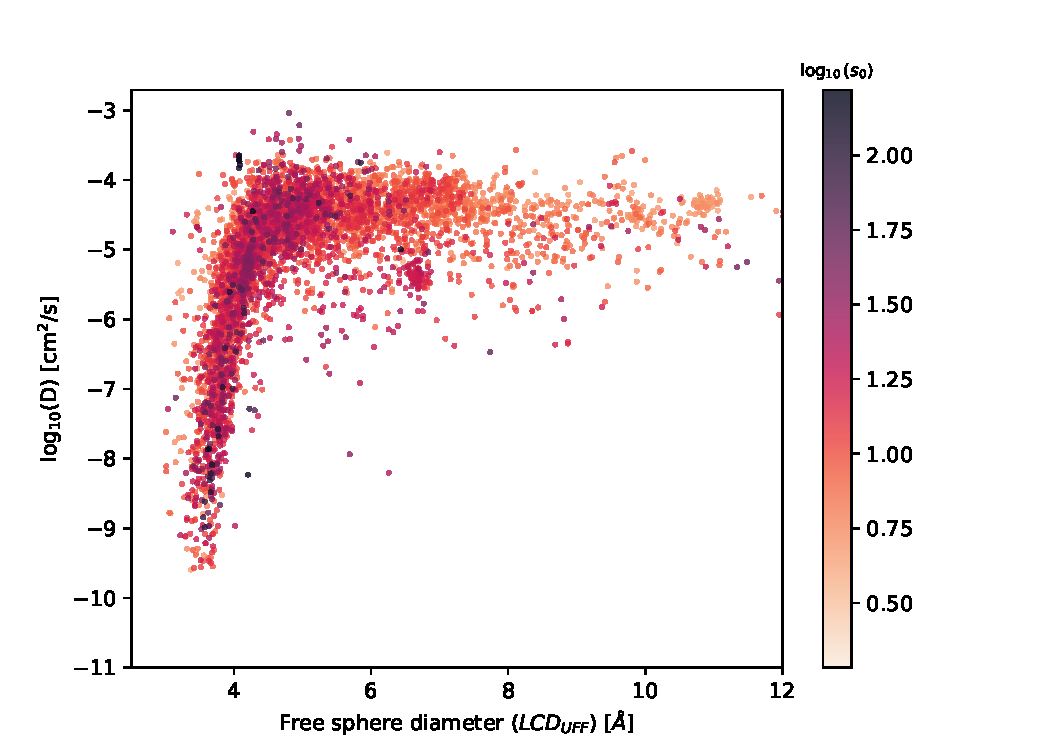
\includegraphics[width=0.48\textwidth]{figures/5-diffusion/D_log-diameter_ccdc_colored_s_+.pdf}
    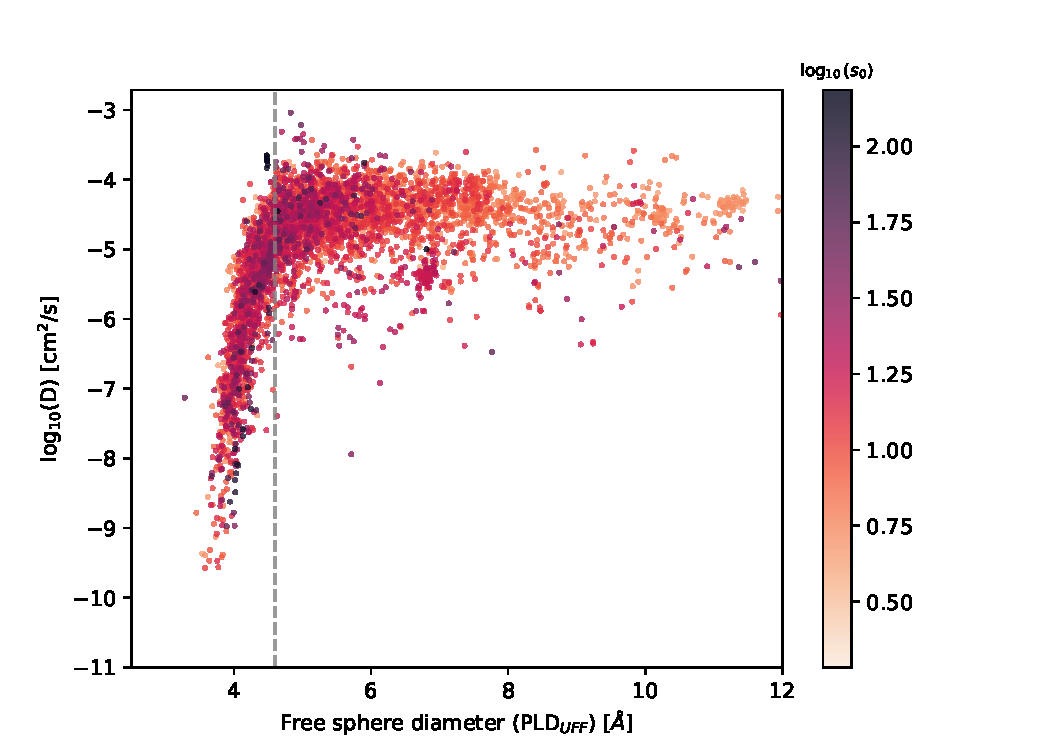
\includegraphics[width=0.48\textwidth]{figures/5-diffusion/D_log-diameter_colored_s_+.pdf}
    \caption{Xenon diffusion coefficient at infinite dilution as a function of the pore limiting diameter (PLD). The diameter of the largest free sphere is defined using two different radius systems: the standard CCDC-based PLD (on the left), and the one defined using the UFF forcefield (on the right)\autocite{Hung_2021} --- as defined in the chapter 2. }\label{fgr:diff_pld}
\end{figure}

If I now analyze the channel dimensions (determined using Zeo++) that could partially inform us on the channel shape. As shown on the Figure~\ref{fgr:scatter_diffusion_chandim}, the dispersion of the diffusion coefficients at the plateau is actually very hard to characterize using the channel dimension with bear eyes. 

\begin{figure}[ht]
  \centering
    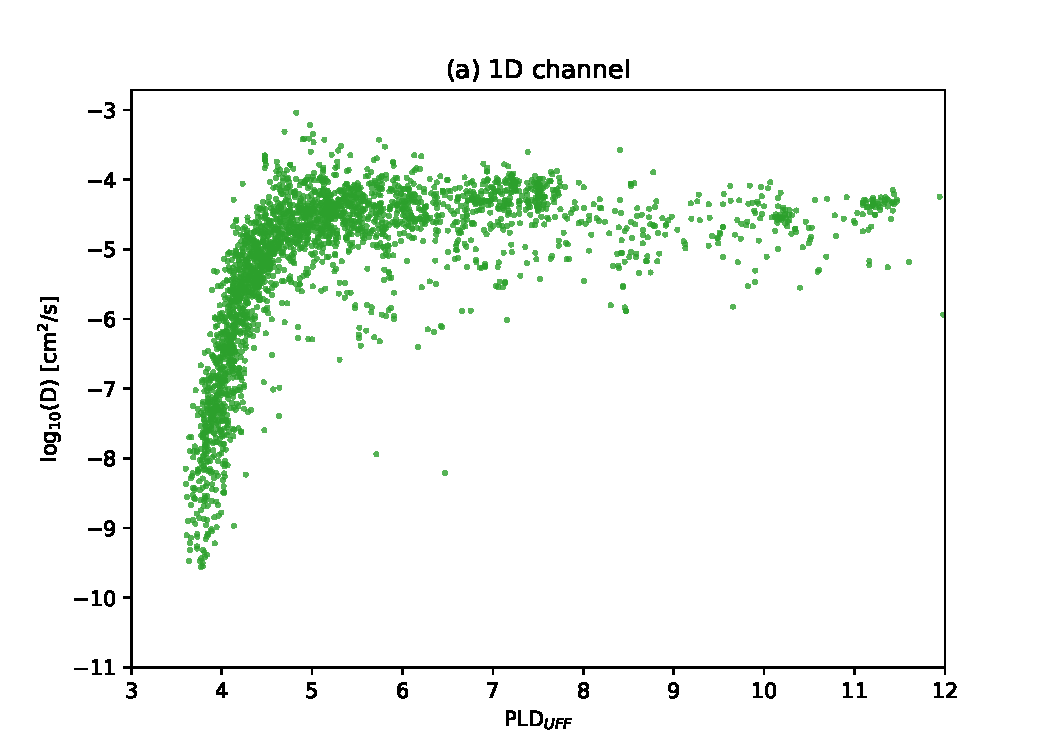
\includegraphics[width=0.32\textwidth]{figures/5-diffusion/D_log-PLD_1D_chan.pdf}
    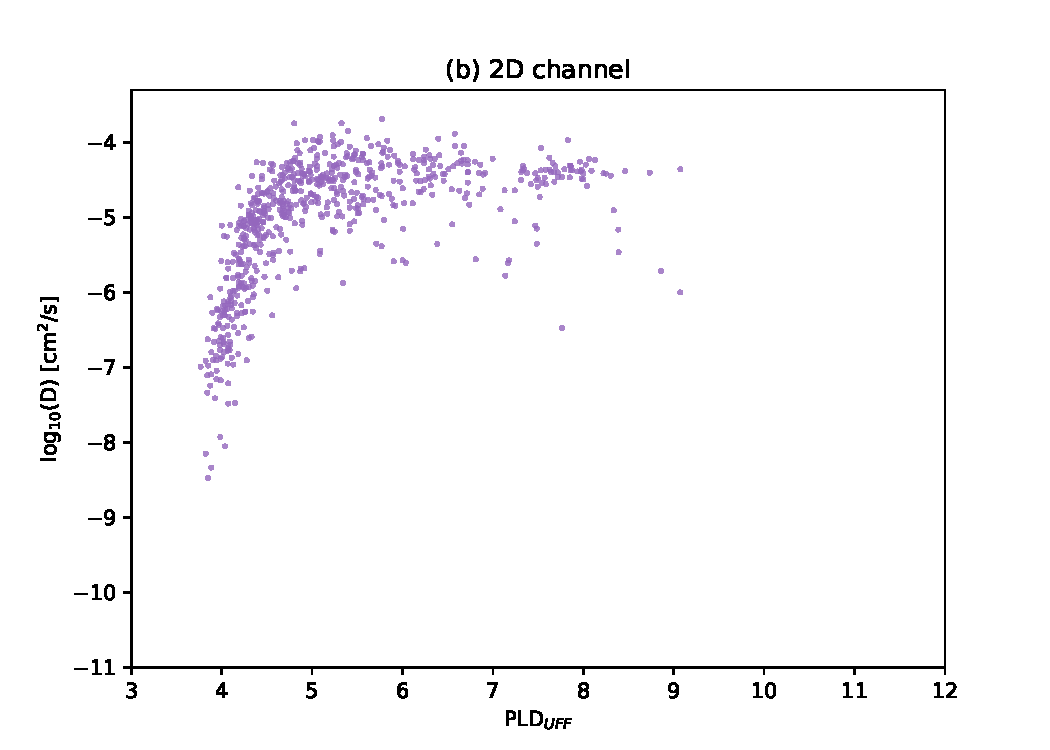
\includegraphics[width=0.32\textwidth]{figures/5-diffusion/D_log-PLD_2D_chan.pdf}
    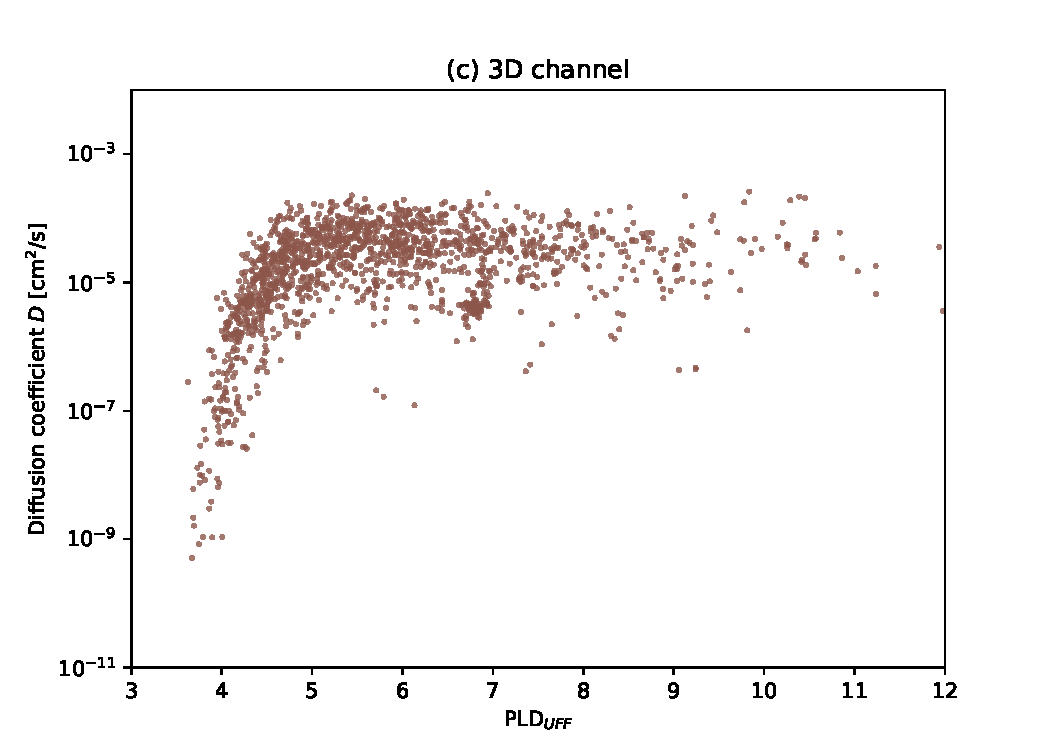
\includegraphics[width=0.32\textwidth]{figures/5-diffusion/D_log-PLD_3D_chan.pdf}
    \caption{ Distributions of the base-10 logarithm of the diffusion coefficients of three different subsets of the screened structures. The first one (a) is composed of structures with a unidimensional channels, the second (b) bidimensional channels and the third one (c) tridimensional channels. }\label{fgr:scatter_diffusion_chandim}
\end{figure}

For this reason, I plotted on the Figure~\ref{fgr:hist_diffusion_chandim} the distribution of diffusion coefficients that depends on the dimensionality of the channels within the framework. The distribution for structures containing 1D structures is much more heavy tail in terms of low diffusion coefficients. We can more easily find 1D structures with very low diffusion coefficients under $3\times 10^{-8}$~\si{\square\cm\per\s}. The vast majority of structures with tridimensional channels has a rather higher diffusion coefficient between $3\times 10^{-6}$~\si{\square\cm\per\s} and $10^{-4}$~\si{\square\cm\per\s} with almost no structures with lower diffusion coefficients. This is not as blatant for bi- and unidimensional channels, we can more easily find structures between $3\times 10^{-8}$~\si{\square\cm\per\s} and $3\times 10^{-6}$~\si{\square\cm\per\s}, even if thery are not that frequent. The dimensionality of the channels can therefore influence the values of diffusion coefficient but the relation is not as clear as for PLD.

\begin{figure}[ht]
  \centering
    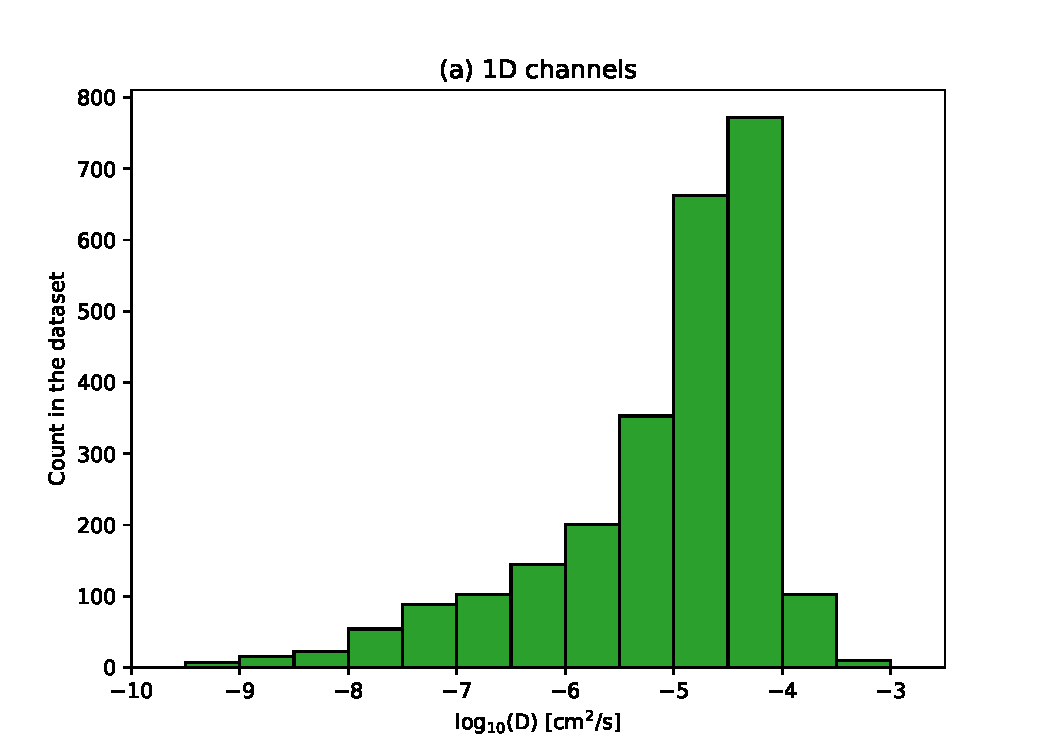
\includegraphics[width=0.32\textwidth]{figures/5-diffusion/histogram_chan1D.pdf}
    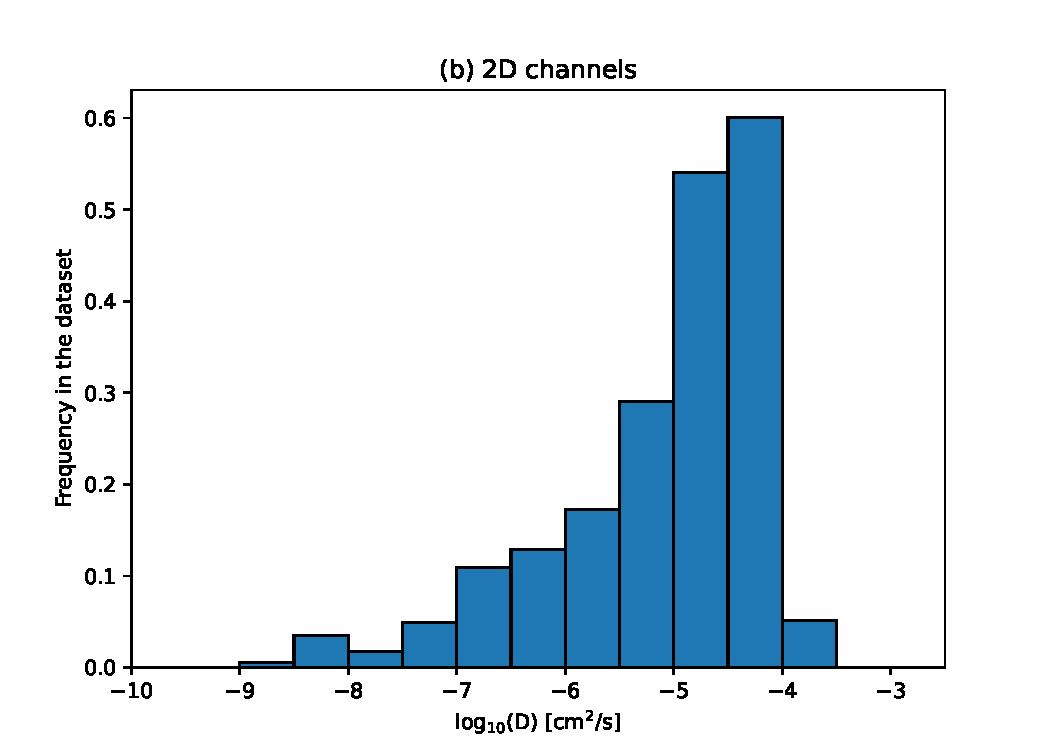
\includegraphics[width=0.32\textwidth]{figures/5-diffusion/histogram_chan2D.pdf}
    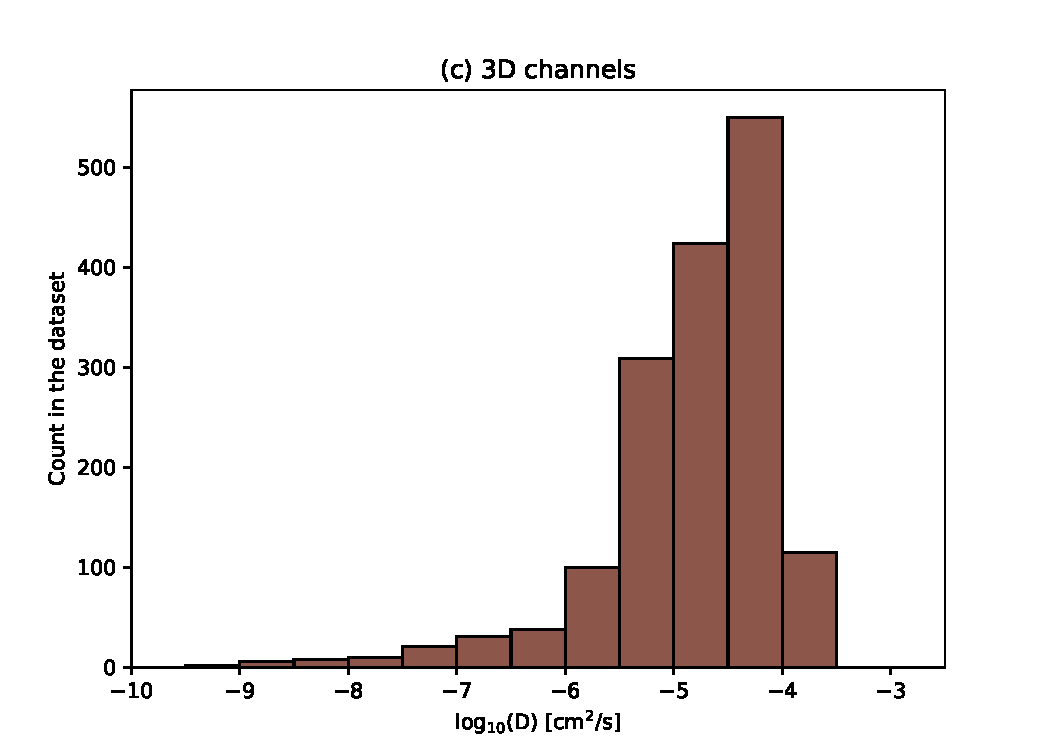
\includegraphics[width=0.32\textwidth]{figures/5-diffusion/histogram_chan3D.pdf}
    \caption{ Distributions of diffusion coefficient of three different subsets of the screened structures. The first one (a) is composed of structures with a unidimensional channels, the second (b) bidimensional channels and the third one (c) tridimensional channels. }\label{fgr:hist_diffusion_chandim}
\end{figure}

Other geometrical properties of the material that can influence the diffusion is the void fraction and surface area. The low diffusion coefficients usually happen in materials with small pore volumes below $0.6$ as shown on the Figure~\ref{fgr:diff_sa_vf}. However, it is diffuscult to draw a relationship between the voide fraction and the diffusion coefficient. The only relation is that materials with void fraction higher than $0.6$ have a diffsion coefficient over $3\times 10^{-6}$~\si{\square\cm\per\s}. This phenomenon is certainly du to the correlation between the PLD and the void fraction. Large PLD values are usually associated with large values of the void fraction. On the other hand, the accessible surface area for a probe of size $1.2$~\si{\angstrom} does not seem to influence the diffusion coefficient at all. 

\begin{figure}[ht]
  \centering
    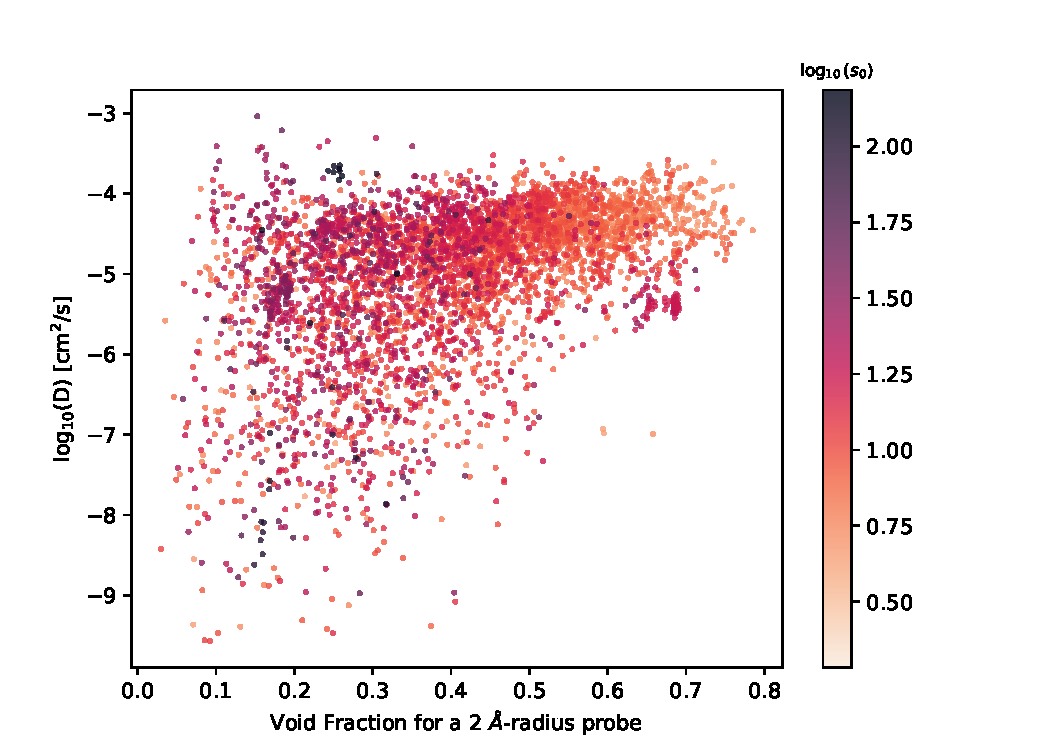
\includegraphics[width=0.48\textwidth]{figures/5-diffusion/D_log-vf_2_s_+.pdf}
    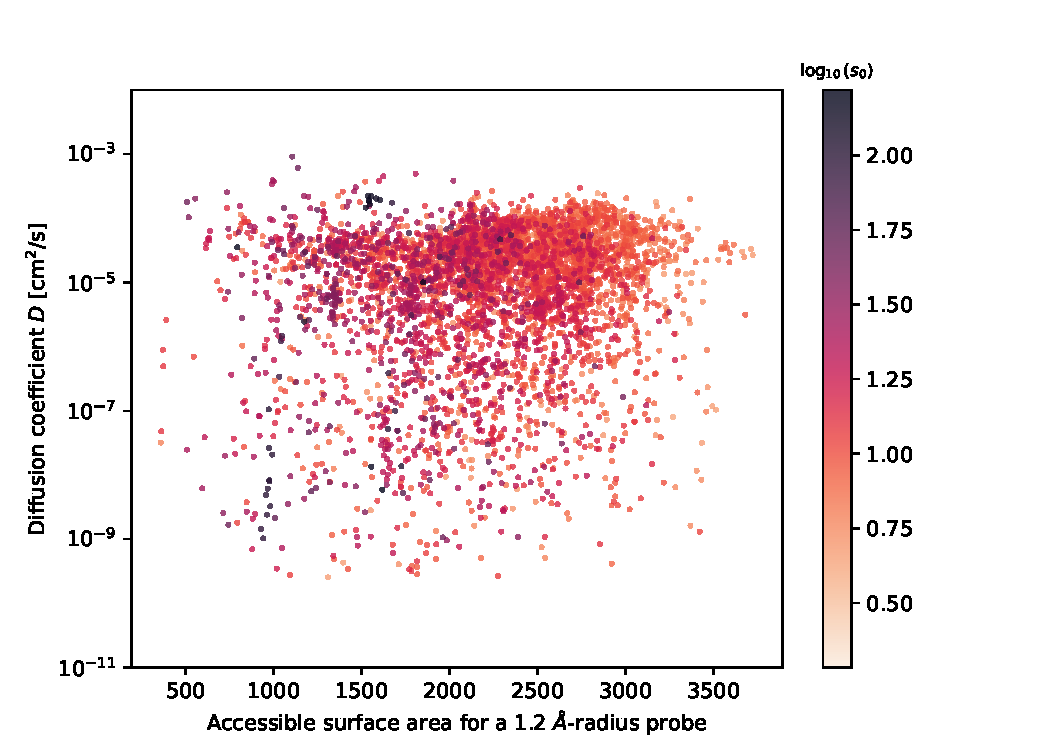
\includegraphics[width=0.48\textwidth]{figures/5-diffusion/D_log-sa_12_s_+.pdf}
    \caption{Xenon diffusion coefficient at infinite dilution as a function of the accessible surface area (left) and the void fraction (right). }\label{fgr:diff_sa_vf}
\end{figure}

Framework density and molar mass are immediate characterictics of the structure since they do not require complicated simulations to obtain. The relation to the diffusion is, however, not that clear on the Figure~\ref{fgr:diff_density_mass}. We can probably say that low values of the density favors high values of the diffusion coefficeint, this can be understtod by the logical relation between low density and high porosity. Another relation to the diffusion coefficient concerns the higher probability to find high diffusion coefficients as materials have a higher molar mass. This last assertion is harder to justify using simple geometrical reasoning. 

\begin{figure}[ht]
  \centering
    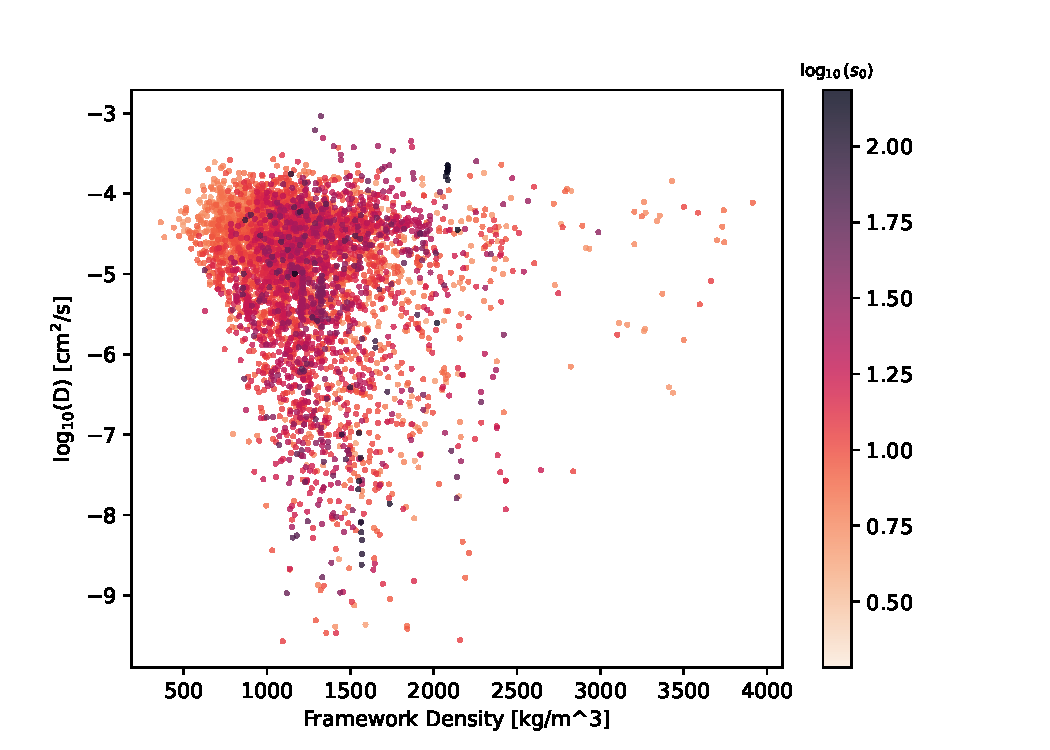
\includegraphics[width=0.48\textwidth]{figures/5-diffusion/D_log-density_s_+.pdf}
    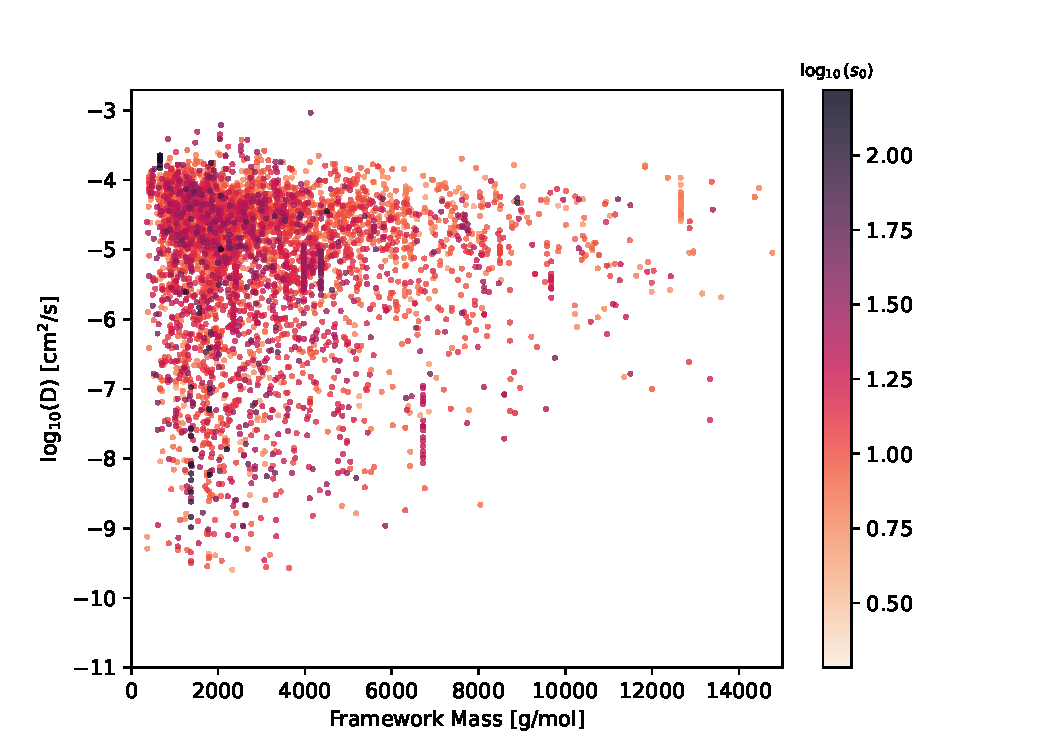
\includegraphics[width=0.48\textwidth]{figures/5-diffusion/D_log-mass_s_+.pdf}
    \caption{Xenon diffusion coefficient at infinite dilution as a function of the density (left) and the mass (right) of the frameworks. }\label{fgr:diff_density_mass}
\end{figure}

The largest sphere diameter D$_{if}$ along a free diffusion path has a similar relation to the diffusion coefficient, but the correlations are much more noisy on the left plot of the Figure~\ref{fgr:diff_H_lcd}.  This can be explained by the fact that D$_{if}$ is always superior or equal to the pore limiting diameter  D$_{f}$ by definition. When both are equal it is equivalent to the Figure~\ref{fgr:diff_pld} with a linear relation and plateau, but if it is higher it creates the sort of noise that we see on the the left plot of the Figure~\ref{fgr:diff_H_lcd}. 

\begin{figure}[ht]
  \centering
    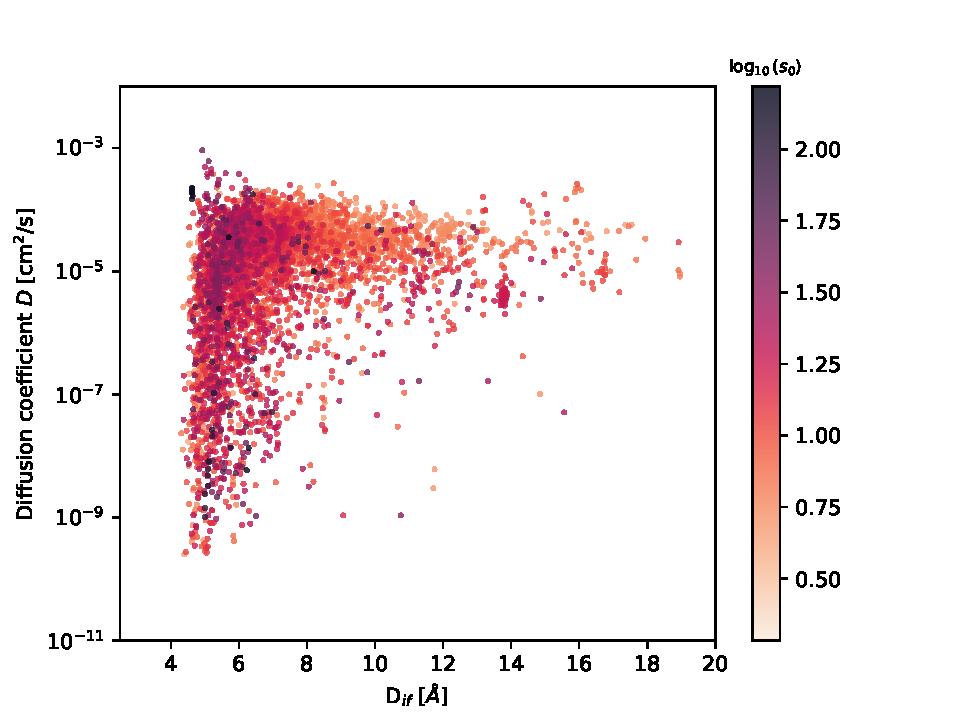
\includegraphics[width=0.48\textwidth]{figures/5-diffusion/D_log-lcd_s_+.pdf}
    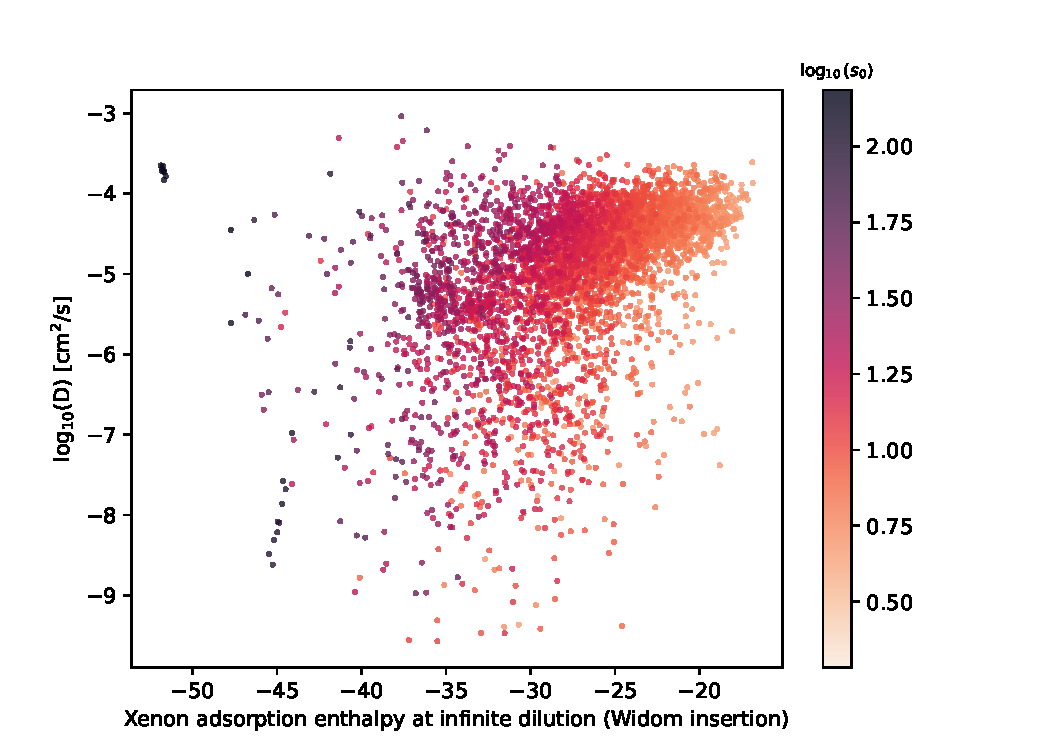
\includegraphics[width=0.48\textwidth]{figures/5-diffusion/D_log-H_Xe_s_+.pdf}
    \caption{Xenon diffusion coefficient at infinite dilution as a function of the largest sphere diameter D$_{if}$ along a free diffusion path (left) and the xenon adsorption enthalpy (right). }\label{fgr:diff_H_lcd}
\end{figure}

The last comparison is made with a thermodynamic quantity, the xenon adsorption enthalpy $\Delta\e{ads}\ex{Xe}H$. There is no relation between diffusion coefficient and the xenon adsorption enthalpy, which is good thing because it means that any configurations are possible. A material can both have a high diffusion coefficient and a high xenon adsorption affinity (very negative values of enthalpy), which is the best configuration for adsorption at infinite dilution. However, it also means that we need to test the diffusivity when the material has a good affinity in order to optimize both properties. This approach will constitue the core discussion around the optimization of both the Xe/Kr selectivity and the diffusion coefficients of Xe and Kr.  

\subsection{A trade-off between the selectivity and the diffusion}

In this section, I will analyze the screening of the diffusion and selectivity properties calculated for xenon and krypton to identify interesting materials that presents both a good Xe/Kr selectivity and a good Xe/Kr diffusion coefficient ratio. To do so I also performed a diffusion coefficient screening for krypton, and I end up with 4,816 structures that has good determination coefficient for both linear fits of xenon and krypton MSD. These structures are then tested to find materials with a good balance between thermodynamic and kinetic properties for the xenon/krypton separation.

\subsubsection{Screening of diffusion selectivity values: a trade-off between adsorption and diffusion}\label{sct:diff_screen}

I will start by comparing the xenon/krypton selectivity at infinite dilution with the xenon and krypton diffusion coefficients. A highly selective materials can have a decent diffusion coefficient, the diffusion limitation observed on the KAXQIL structure is therefore not inevitable, which is a good news. On the left plot of the Figure~\ref{fgr:diff_s0_lcd}, we can clearly see that all configurations are possible: high selectivity (over $40$) with high diffusion coefficient (over $10^{-6}$~\si{\square\cm\per\s}) and high selectivity with low diffusivity. The krypton coefficients seem to be rather stable between $10^{-6}$~\si{\square\cm\per\s} and $10^{-3}$~\si{\square\cm\per\s}. It means that it is not the main leverage to increase the diffusion selectivity since very low values of kryton diffusion coefficients do not appear for highly selective materials. To go beyond the thermodynamic selectivity, I will study a transport related selectivity metric to find highly selective materials that do not show significant transport limitations.

\begin{figure}[ht]
  \centering
    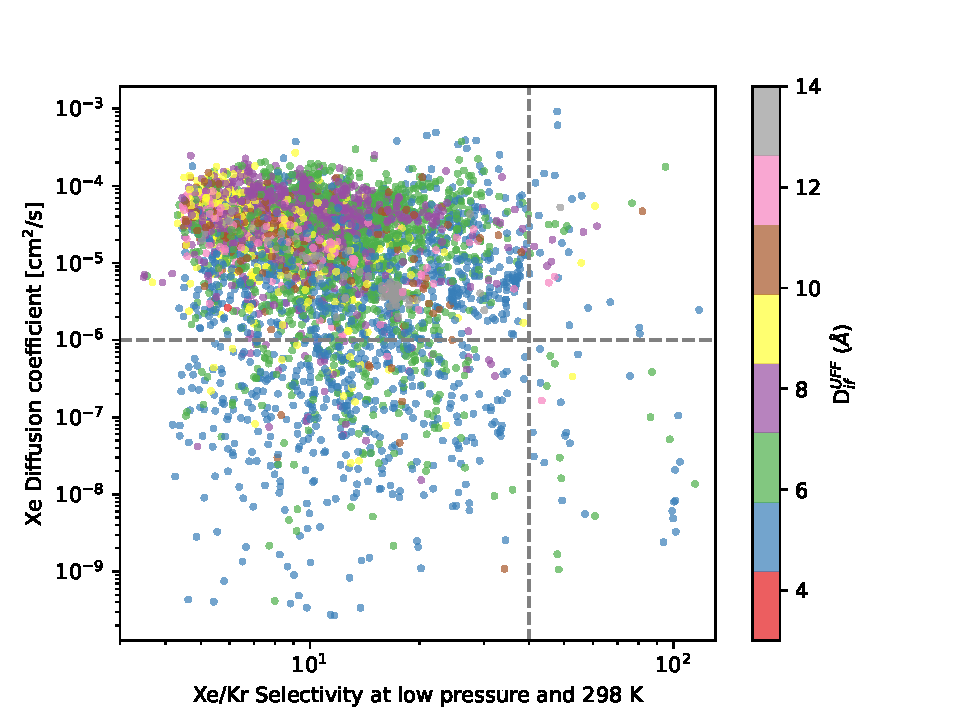
\includegraphics[width=0.48\textwidth]{figures/5-diffusion/D_xe-s0-lcd.pdf}
    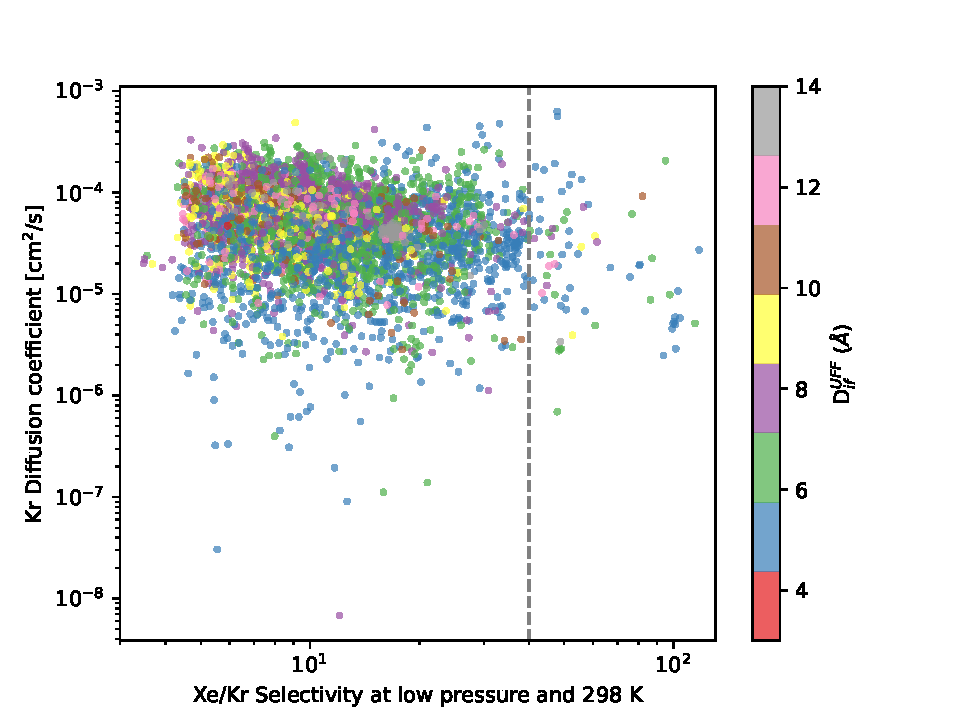
\includegraphics[width=0.48\textwidth]{figures/5-diffusion/D_kr-s0-lcd.pdf}
    \caption{}\label{fgr:diff_s0_lcd}
\end{figure}

To take account of the transport properties in a separation process, we generally use the ratio of the diffusion coefficients or the diffusion selectivity as a performance metric. For xenon and krypton the diffusion selectivity can be defined as follows:\autocite{Krishna_2010}
\begin{equation}
  s\ex{Xe/Kr}\e{diff} = \frac{D\ex{Xe}}{D\ex{Kr}}
\end{equation}
If we want to look at both the transport and thermodynamic effects, we can combine the thermodynamic adsorption selectivity defined in chapter 2 (equations~\ref{eq:selec_0} and~\ref{eq:selec_0}) and the diffusion selectivity to define the membrane selectivity (used to characterize membranes). This membrane selectivity can also be called a perm-selectivity because it corresponds to the ratio of the permeabilities of the components of the binary mixture we want to separate. The xenon/krypton permselectivity $s\ex{Xe/Kr}\e{perm}$ can therefore be defined as follows:
\begin{equation}\label{eq:membrane_selec}
  s\ex{Xe/Kr}\e{perm} = s\ex{Xe/Kr}\e{diff} \times s\ex{Xe/Kr}\e{ads}
\end{equation}
where $s\ex{Xe/Kr}\e{ads}$ corresponds to the adsorption selectivity used throughout the previous chapters (at infinite dilution or higher pressure). 

\begin{figure}[ht]
  \centering
    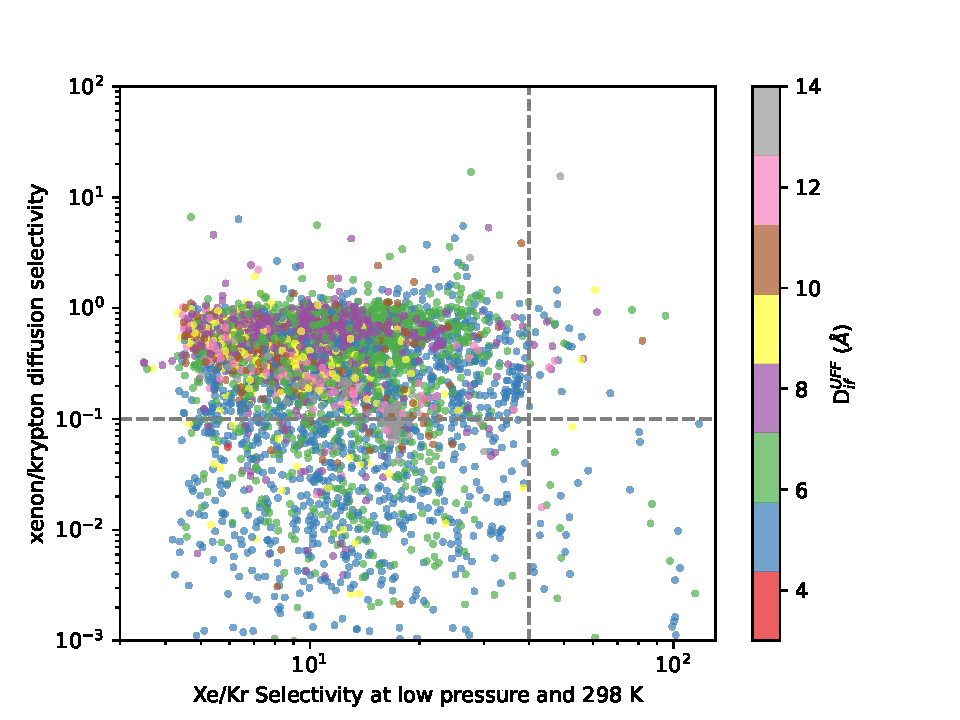
\includegraphics[width=0.48\textwidth]{figures/5-diffusion/diff_D_xekr-s0-lcd.pdf}
    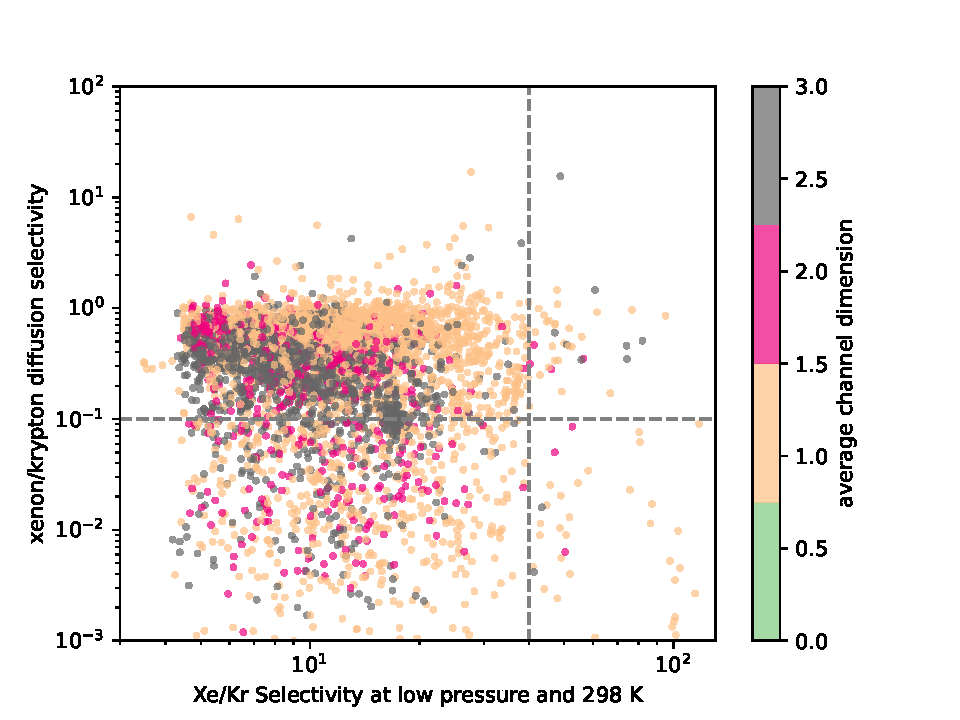
\includegraphics[width=0.48\textwidth]{figures/5-diffusion/diff_D_xekr-s0-chandim.pdf}
    \caption{}\label{fgr:perm_selec0}
\end{figure}

Using both $s\ex{Xe/Kr}\e{diff}$ and $s\ex{Xe/Kr}\e{ads}$ at different pressure conditions, I will try to find materials that exhibit a rather high selectivity with a high diffusion selectivity. The plots of the Figure~\ref{fgr:perm_selec0} shows that 48 structures have a selectivity over $40$ with a rather good diffusion selectivity over $0.1$. These structures have rather high values of pore size represented by the largest included sphere along a free diffusion path $D_{if}$ as shown on the left plot of the Figure~\ref{fgr:perm_selec0}. And these rather large pores are associated with structures with different dimensionalities.
One remarkable structure among them has a very high diffusion selectivity (over $15$, grey point on the upper right side of the left plot of Figure~\ref{fgr:perm_selec0}) coupled with a high adsorption selectivity at infinite dilution. This structure, with a CSD code ADOGEH\cite{Peikert_2012}, has a tridimensional channel framework with large pores and rather narrow connecting channels. The high adsorption selectivity at infinite dilution is however not conserved at ambient pressure as shown on the Figure~\ref{fgr:perm_selec2080}  (see Table~\ref{table:diff}).

If we look into the details of these structures, we can see that they combine large pores with smaller pores so that the diffusion is not obstructed and the selectivity is high in more confined spaces. These type of materials with different sizes of pore could cause a selectivity drop at higher pressure, because the larger pores are less selective and are accessed when the gas pressure is increased. This phenomenon is observed when comparing the plots to the ones of Figure~\ref{fgr:perm_selec2080}.

\begin{figure}[ht]
  \centering
    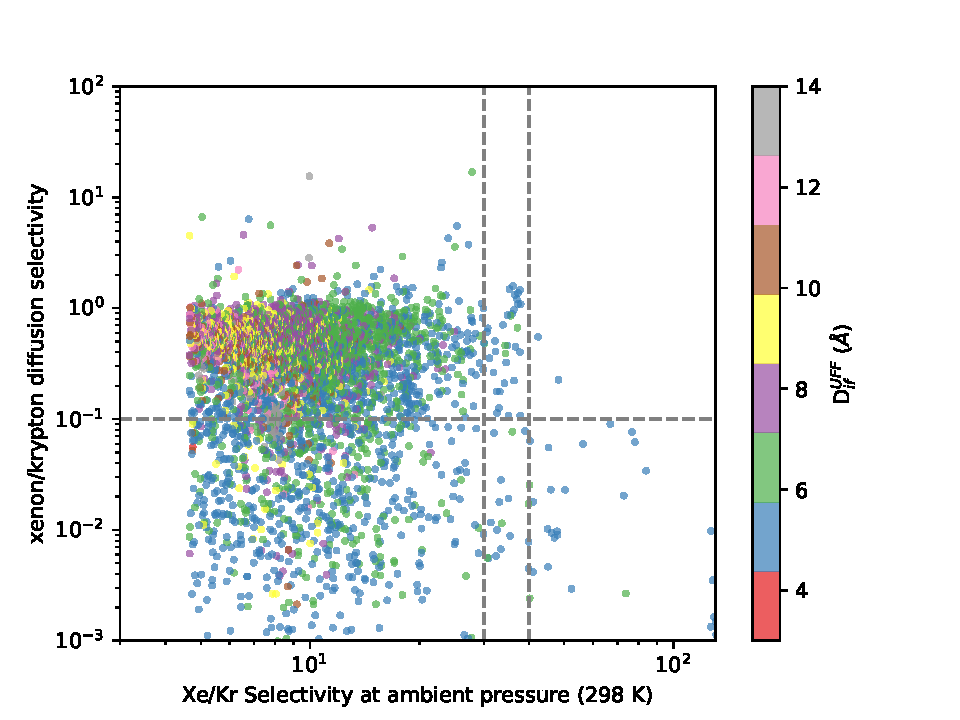
\includegraphics[width=0.48\textwidth]{figures/5-diffusion/diff_D_xekr-s2080-lcd.pdf}
    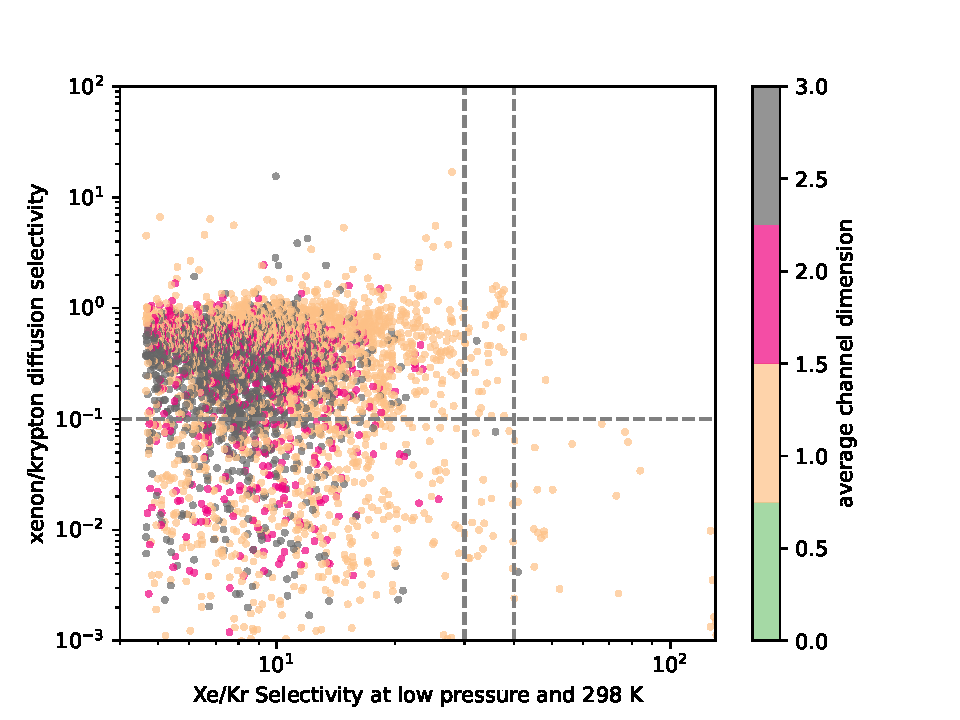
\includegraphics[width=0.48\textwidth]{figures/5-diffusion/diff_D_xekr-s2080-chandim.pdf}
    \caption{}\label{fgr:perm_selec2080}
\end{figure}


We can see that at higher pressure, some materials experience a shift toward lower selectivity values. And, only 2 structures have an ambient-pressure selectivity over $40$: the MOFs with the following CSD code XUNSOQ\autocite{Abrahams_2014} and GUMDEZ\autocite{Yin_2014}  (see Table~\ref{table:diff}). Most of these materials actually have a high value of cavity size, only structures with LCD near \SI{6}{\angstrom} are left in this area of the plot. We can also note that the dimension of the channel is equal to one too, which starts to brush a picture of the interesting materials. These materials are constituted of unidimensional channels with a small pore sizes so that the selectivity is conserved even at higher pressure conditions. If we broaden the scope to the structures with a selectivity higher than $30$ instead of $40$, we now have 38 structures that also have similar features with rather low pore sizes and low channel dimensionality. Some of these structures have more or less kept their selectivity such as QOZDOY\autocite{Zhang_2001} and wasn't detected on the pre-screening on the low-pressure selectivity (Figure~\ref{fgr:perm_selec0}), but other structures, such as the MOF MISQIQ\autocite{Tong_2013}, actually dropped significantly in selectivity values from infinite dilution to ambient pressure (see Table~\ref{table:diff}). 

When considering the ambient-pressure selectivity, the large majority of highly selective materials actually have a rather low diffusion selectivity (lower than $0.1$), as shown on the Figure~\ref{fgr:perm_selec2080} (this was not the case for the low-pressure selectivity). This result suggest that a trade-off between adsorption selectivity and diffusion selectivity is actually needed. In my screening approach, I decided to lower the adsorption diffusivity to values around $40$ to allow for higher diffusion selectivity values, because up until now standard screenings in the literature\autocite{Simon_2015,Chung_2019} and in my published work~\cite{Ren_2021} only mazimized the adsorption selectivity --- this equivalent to working on the lower right side of the plots of Figure~\ref{fgr:perm_selec2080}. To improve the former approach, I included a kinetic constraint in our screening. Another approach would be to optimize the perm-selectivity also known as the membrane selectivity (equation~\ref{eq:membrane_selec}), but it would be the solution to another application, the membrane separation, which is broadly studied in the literature\autocite{Anderson_2017,Wang_2022}. In the screening I presented here, we would like to find thermodynamically selective materials that are not limited by diffusion, and some interesting identified materials will be further studied in the following subsection. 


\subsubsection{Identification of interesting materials}

By crossing the transport data with the thermodynamic one, we can optimize the Xe/Kr adsorption selectivity under some constraint on the diffusion selectivity so that it is in an acceptable range (over $0.1$). The structures of the 65 structures with a low-pressure Xe/Kr selectivity higher than $40$ or with an ambient-pressure Xe/Kr selectivity higher than $30$ have been manually visualized and quickly analyzed, and different materials have been hand-picked for further analysis due to some special characterictics. I discarded some materials that have different type of channels that can artificially have a high diffusion coefficient. This phenomenon is due to the randomness of the initial condition, for example, when the xenon diffuses in a wider channel while the krypton diffuses in the narrower channel, the diffusion selectivity will inevitability be artificially higher. For example, the MOF with a CSD code OQESAF\autocite{Xie_2011} was concerned by this phenomenon as shown on the Figure~\ref{fgr:OQESAF} it clearly has different diffusion coefficeint values depending on the channel considered (a Henry coefficient weighted average need to be performed in this case). Other materials have a moderately high diffusion selectivity ($\lesssim 1$), they are usually composed of a unidimensional channel that allows a rather free diffusion of a xenon (higher than \SI{4.6}{\angstrom}) with different cavity sizes. Different factors seem to influence the diffusion coefficients, the values of the channel size and the pore size could explain the values of the diffusion and adsorption selectivity, but more interestingly the shape of the channel composed of cavities connected by narrower walls is also very important. Depending on the tortuosity of the layout and the relative difference between the cavities and the connecting channels, diffusion properties can be very different. 

\begin{figure}[ht]
  \centering
    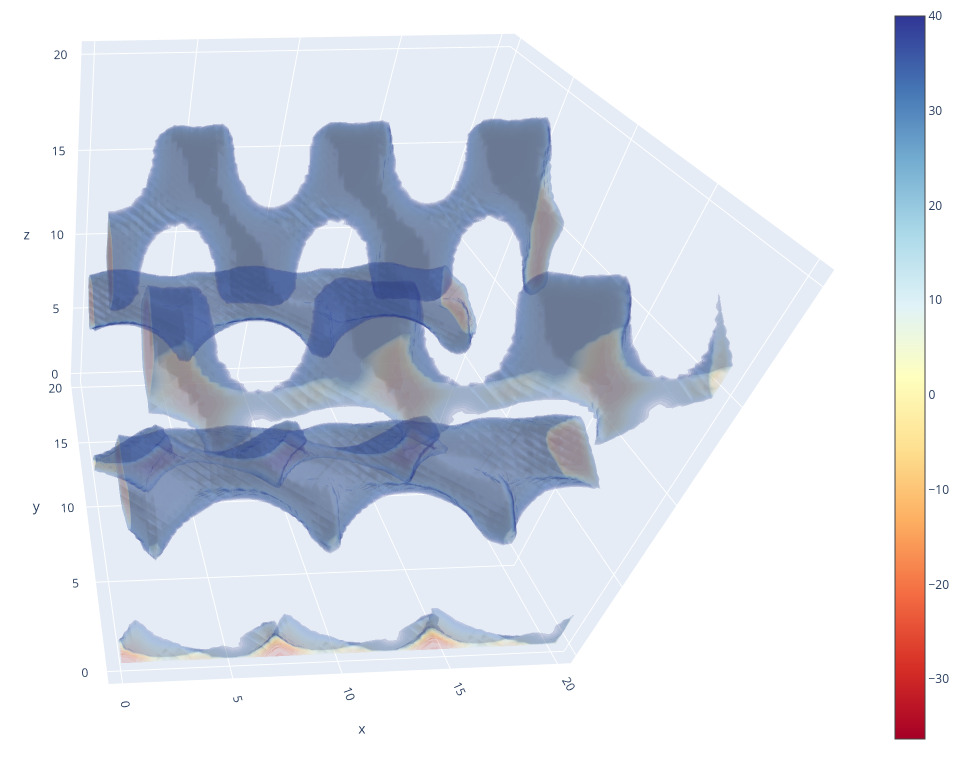
\includegraphics[height=0.4\textwidth]{figures/5-diffusion/viz/OQESAF.jpg}
    \caption{Snapshot of a 3D visualization of the xenon interaction energy inside the channels of the OQESAF\autocite{Xie_2011} material. We can see two different unidimensional channels. In an MD simulation of a single xenon per box, we cannot test out all the initial positions. }\label{fgr:OQESAF}
\end{figure}

In this section, I will look into the details of the comparative transport and adsorption performances of some archetypal structures (Table~\ref{table:diff}) to better understand the key factors that could explain the difference in performance. In the future, this work can be used for the design of more quantitative characteristics that could explain the better transport performance, similarly to what I did for the thermodynamic screening that led to a series of key thermodynamic descriptors that led to the design of a ML model for adsorption selectivity prediction (chapters 3--4). To achieve this, I will use a visualization tool based on the grid calculation principle shown in the dedicated section~\ref{sct:grid}, and the code is published in the same Github repository: \url{github.com/coudertlab/GrAED}.

\begin{table}[ht]
\small
\setlength\extrarowheight{2pt}
\centering
\begin{tabular}{|l|c|c|c|c|c|c|c|}
\hline
  Structure &       &    &  Pore size &  Channel size   &     & Diffusion Coeff. & Xe uptake \\
  CSD ref.\ code &  $s_0\ex{Xe/Kr}$  &  $s_1\ex{Xe/Kr}$   &    D$_{if}\ex{UFF}$ (\si{\angstrom})   &   PLD\ex{UFF} (\si{\angstrom})  &  $s\e{diff}\ex{Xe/Kr}$ &  $D\e{diff}\ex{Xe}$ (\si{\square\centi\meter\per\second}) & (\si{\milli\mole\per\gram}) \\
\hline
OQESAF~\cite{Xie_2011} & 28 & 28 &  5.8 & 5.0 &  17 &  4$\times$10\ex{-5} & 3.2 \\
\hline
ADOGEH~\cite{Peikert_2012} & 49  &  10 & 12.9 & 5.3 & 15.5 &  5$\times$10\ex{-5} & 1.7 \\
\hline
KAXQIL~\cite{Banerjee2012} & 104  & 133 &  5.2 & 4.1 &  0.005 &  3$\times$10\ex{-8}  & 1.4 \\
XUNSOQ~\cite{Abrahams_2014} & 38  & 48 &  5.6 & 4.8 &  0.23 &  7$\times$10\ex{-6} & 3.5 \\
BAEDTA01~\cite{Chen_2010} & 152 & 38 &  5.7 & 4.6 &  0.4 &  4$\times$10\ex{-5} & 1.1 \\
TONBII~\cite{Du_2010} & 44 & 35 &  5.1 & 4.8 &  0.86 &  1$\times$10\ex{-4} & 1.5 \\
\hline
VOHQIS~\cite{Wragg_2001} & 51 & 48 &  5.7 & 3.9 &  0.01 &  6$\times$10\ex{-8} & 2.6\\
QOZDOY~\cite{Zhang_2001} & 52  & 37 &  5.6 & 5.0 &  0.45 &  7$\times$10\ex{-5} & 3.7 \\
GUMDEZ~\cite{Yin_2014} & 56 & 42 &  5.5 & 5.1 &  0.55 &  7$\times$10\ex{-5} & 3.0 \\
MISQIQ~\cite{Tong_2013} & 140 & 37 &  4.6 & 4.5 &  1.4 &  2$\times$10\ex{-4} & 2.3 \\
\hline
\end{tabular}
\caption{Transport and thermodynamic performances of top performing structures of CoRE MOF 2019 screened out by the approach developed in section~\ref{sct:diff_screen}. The thermodynamic properties are determined using xenon uptake at \SI{1}{\bar} and \SI{298}{\kelvin}, $s_0\ex{Xe/Kr}$ and $s_1\ex{Xe/Kr}$ that correspond to the xenon/krypton adsorption selectivity values respectively at infinite dilution and ambient pressure condition. The pore size is defined as the largest cavity along a free diffusion path D$_{if}\ex{UFF}$ and the channel size is defined using the pore limiting diameter PLD\ex{UFF} using atom radii defined by the UFF. The transport properties are evaluated using the xenon/krypton diffusion selectivity $s\e{diff}\ex{Xe/Kr}$ and the xenon diffusion coefficient $D\e{diff}\ex{Xe}$ calculated by the MD-based screening presented above. }\label{table:diff}
\end{table}

The structure ADOGEH\autocite{Peikert_2012} was not found when crossing the transport data with ambient-pressure selectivity values by with the infinite dilution ones, which explains that the selectivity $s_1$ is rather low ($10$) compared to the other materials (over $35$). This structure was actually detected when looking at the selectivity $s_0$ at infinite dilution, because of its extraordinary diffusion selectivity around ($10$). This would mean that as membrane material, its selectivity would be around $100$, which is on of the highest. Even as an adsorption-based separation material, it has an outstanding low-pressure selectivity of $49$ coupled with the high diffusion selectivity it can be considered for some applications at very low partial pressure of xenon and krypton. 

\begin{figure}[ht]
  \centering
  \begin{subfigure}[b]{0.4\textwidth}
    \centering
    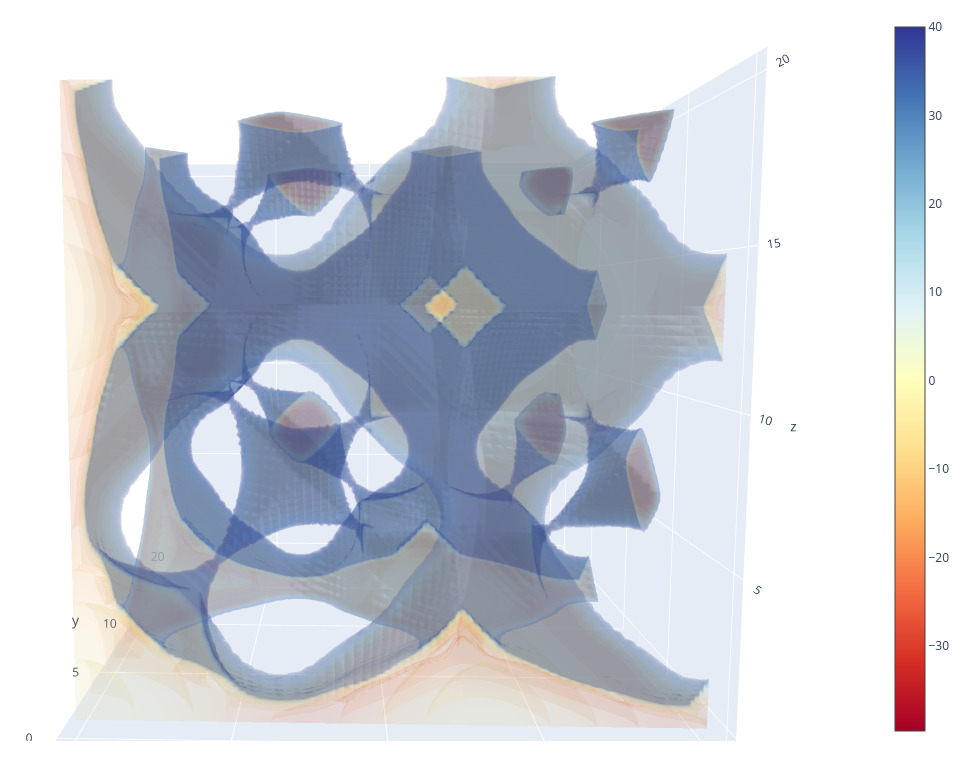
\includegraphics[width=\textwidth]{figures/5-diffusion/viz/ADOGEH_Xe.jpg}
    \caption{Xe energy grid in ADOGEH}\label{fgr:ADOGEH_Xe}
  \end{subfigure}
  \hspace{1cm}
  \begin{subfigure}[b]{0.4\textwidth}
    \centering
    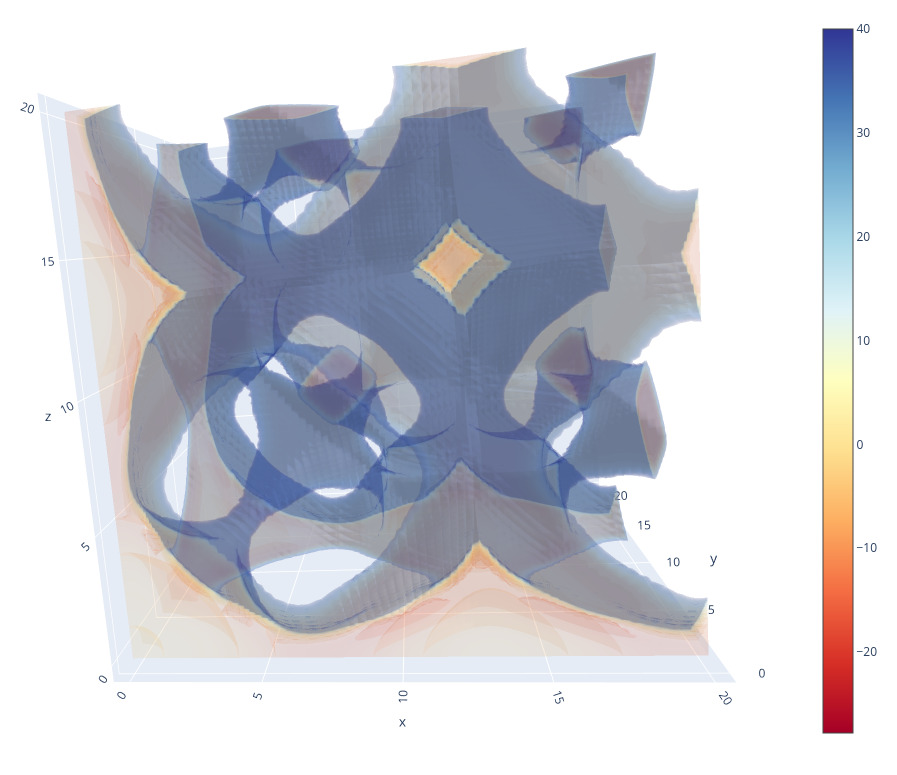
\includegraphics[width=\textwidth]{figures/5-diffusion/viz/ADOGEH_Kr.jpg}
    \caption{Kr energy grid in ADOGEH}\label{fgr:ADOGEH_Kr}
  \end{subfigure}
  \caption{3D volume plot of the xenon (a) and krypton (b) interaction energy values inside the material ADOGEH\autocite{Peikert_2012} calculated using an energy grid as described in section~\ref{sct:grid}. }\label{fgr:ADOGEH}
\end{figure}

And even as an experimental material, the diffusion properties of xenon and krypton in this material are extremely interesting in themselves. On the Figure~\ref{fgr:perm_selec0}, only two materials have a diffusion selectivity over $10$, but the other one actually has a falsely high value of diffusion selectivity due to the above-mentioned randomness of the initial position in the MD simulation and the presence of two types of channel (see Figure~\ref{fgr:OQESAF}). ADOGEH is therefore the only material that shows such a high diffusion selectivity among all materials screened for their diffusion performance. In a unidimensional system, it is actually more natural to have a higher or equivalent diffusion coefficient for krypton than for xenon due to the obvious size difference. 

It is possible to explain this exceptional by a special mechanism that happens in the tridimensional channel network of ADOGEH. As shown on the Figure~\ref{fgr:ADOGEH}, for both xenon and krypton all dimensions are available for diffusion through the channels in the three cardinal directions. However, when we look at the sort of ``pocket'' (not a blocking pocket in the MD simulation) that connects the channels diagonally, the access to it is clearly not the same if we compare the two 3D energy grid plots. For xenon, on the Figure~\ref{fgr:ADOGEH_Xe}, the connection is way thinner than for krypton, on the Figure~\ref{fgr:ADOGEH_Kr}, for the same energy threshold. This can be interpreted as a higher energy barrier for xenon than for krypton to access this ``pocket''. But, why would this explain the unusual difference in diffusion coefficients for xenon and krypton? This can be explained by the fact that the directions in which a krypton can diffuse is therefore much higher, which means that it has a higher probability of turning around than xenon. To say it more explicitely, a xenon can diffuse in the 3D space by taking only 3 main directions, but a krypton would lose time deviating from the cardinal directions --- the same way as opening-up dimensions decreases the diffusion coefficient ($\langle{r(t)}^2\rangle=2d\tau$). Moreover, when a krypton takes the small channel toward the ``pocket'', it would have a non negligible residence time inside, which further slows it down compared to a xenon. These ``pockets'' can be seen as traps for krypton, if it were a race between both adsorbate inside the nanoporous material. 


Beyond the particular cases of OQESAF and ADOGEH, other nanoporous materials have lower diffusion selectivity values. For instance, all the other materials of the Table~\ref{table:diff} have a diffusion selectivity between $0.2$ and $1.4$. Depending on the shape and the size distribution of the porous channels, we would have higher or lower values of diffusion selectivity and xenon diffusion coefficient values. For instance, as shown on the Figure~\ref{fgr:porediff_b}, there seems to be a weak correlation between a pore size characteristics (LCD\ex{UFF}$-$PLD\ex{UFF}) and the diffusion performance for structures with a LCD\ex{UFF} value lower than \SI{6}{\angstrom} --- for these structures, pore size have a higher chance to influence the transport properties. This correlation is logically due to the fact that if this difference between LCD and PLD is high, the diffusing xenon will have to cross a higher energy barrier to move inside the channels, therefore decreasing the diffusion coefficient. If we consider, all structures available, the correlation disappears because in the materials with a higher LCD value the movement of the diffusing xenon is not influenced as much by the pore walls. And actually for values of LCD higher than \SI{7}{\angstrom}, the diffusion coefficient is rather stabilized around $10^{-5}$~\si{\square\cm\per\s} as shown on the Figure~\ref{fgr:diff_H_lcd}. 

For structures with a high ambient-pressure selectivity (Figure~\ref{fgr:porediff_c}), we can now see a negative linear relation between this LCD-PLD difference and the xenon/krypton diffusion selectivity. This is actually due to the fact that highly selective materials have pore size close to the size of a xenon as shown in details in the previous chapters. The effect on Xe diffusion coefficient can in fact be enlarged to the Xe/Kr diffusion seelectivity as previously suggested by the noisy but stable values of Kr diffusion coefficients around $3\times10^{-5}$~\si{\square\cm\per\s} (see Figure~\ref{fgr:diff_s0_lcd}). The weakness of the correlation can be explained by the uncertainty inherent to the MD methodology for diffusion coefficient calculation (evaluated to around {20\%} for the material KAXQIL), but also by phenomena that I did not cover with the simple arithmetic difference of two pore characteristics. For instance the tortuosity of the channel, which is very tricky to evaluate in a tridimensional space can surely add some insight to the comprehension of the diffusion coefficeint values. For instance, I will show different channel shape in the different examples below that can be qualitatively discussed but no effort to quantify these effects have been done in my current work.

\begin{figure}[ht]
  \centering
  \begin{subfigure}[b]{0.32\textwidth}
      \centering
      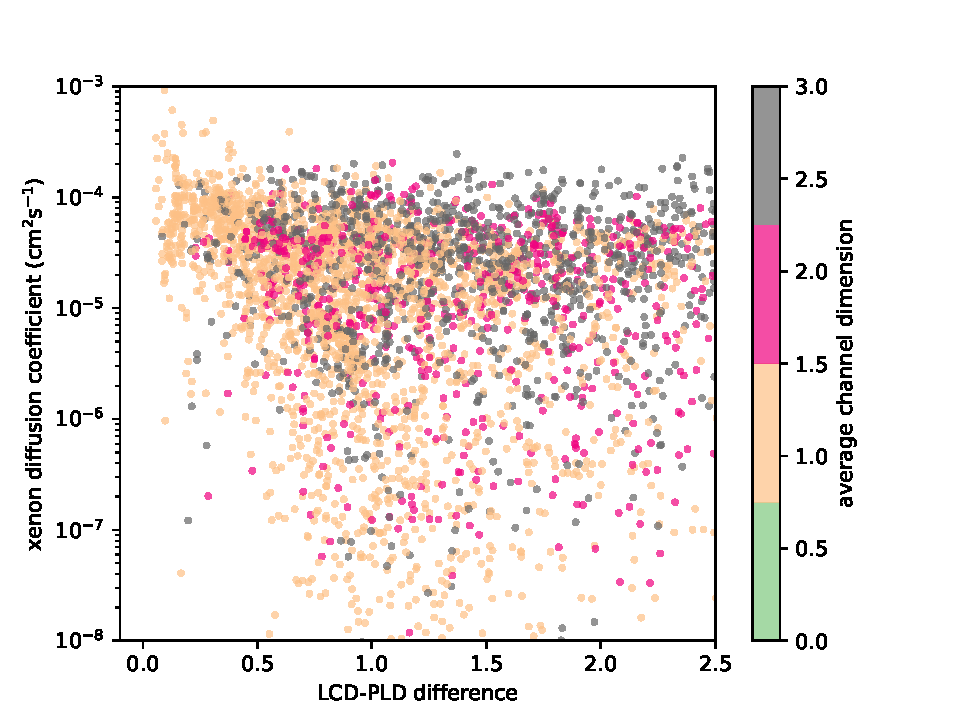
\includegraphics[width=\textwidth]{figures/5-diffusion/D_xe-poresize-chandim_all.pdf}
      \caption{All structures}\label{fgr:porediff_a}
  \end{subfigure}
  \hfill
  \begin{subfigure}[b]{0.32\textwidth}
      \centering
      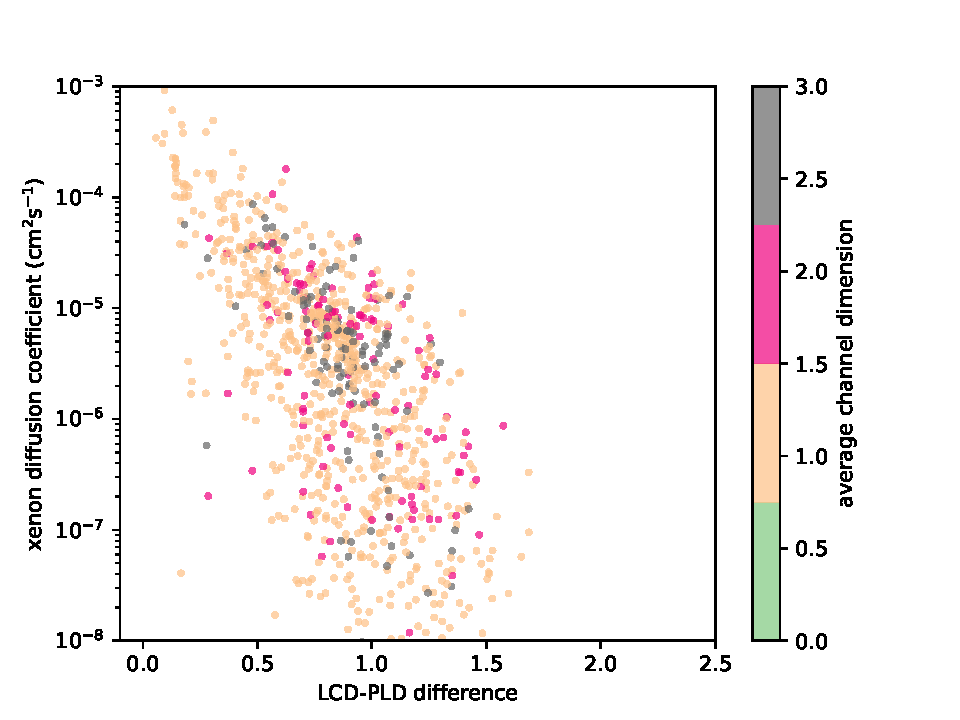
\includegraphics[width=\textwidth]{figures/5-diffusion/D_xe-poresize-chandim_LCDunder.pdf}
      \caption{LCD\ex{UFF}$<5.5$}\label{fgr:porediff_b}
  \end{subfigure}
  \hfill
  \begin{subfigure}[b]{0.32\textwidth}
      \centering
      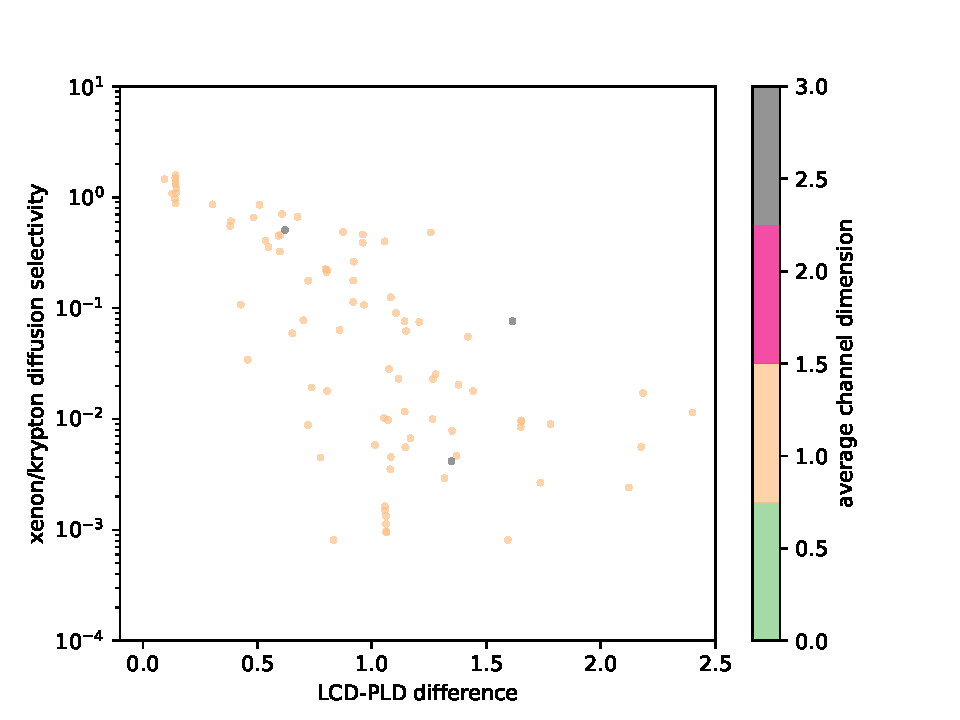
\includegraphics[width=\textwidth]{figures/5-diffusion/diff_D_xekr-poresize-chandim.pdf}
      \caption{$s\ex{Xe/Kr}_1>30$}\label{fgr:porediff_c}
  \end{subfigure}
     \caption{ Scatterplots of the diffusion coefficient compared to the LCD-PLD difference labeled using the channel dimension for all structures (a) and for structures with an LCD above \SI{5.5}{\angstrom} (b). On the subfigure (c), the scatterplot of the xenon/krypton diffusion selectivity compared to the LCD-PLD difference for the most selective structures ($s\ex{Xe/Kr}_1>30$). }\label{fgr:porediff}
\end{figure}

The highly selective materials shown in the Figure~\ref{fgr:porediff_c} are actually shown on the Table~\ref{table:diff}. The negative linear relation between the LCD-PLD difference and the Xe/Kr diffusion selectivity or the Xe diffusion coefficient can be reconfirmed by looking at the values of the Table for materials with 1D channels (ADOGEH excepted). I am now going to split them into two categories in order to take a glimpse on the tortuosity difference between these materials.  

We can first take a look at materials with nanopores composed of pseudo-spherical cavities connected by cylindrical channels following a straight line, as shown on the Figure~\ref{fgr:tube_cavities}. These channels are actually forming straight lines, and if evaluated, their tortuosity would actually be very low. For TONBII, we actually have very small LCD-PLD difference, which explains the rather high diffusion selectivity near $1$. There are almost no difference between xenon and krypton diffusing in the channels of this material. When the value of LCD increases, for a very similar value of PLD, the diffusion selectivity of such materials drops for BAEDTA01 and XUNSOQ as shown on the Table~\ref{table:diff}. This drop can be explained by a now lower value of the xenon diffusion coefficient. 

\begin{figure}[ht]
  \centering
  \begin{subfigure}[b]{0.3\textwidth}
      \centering
      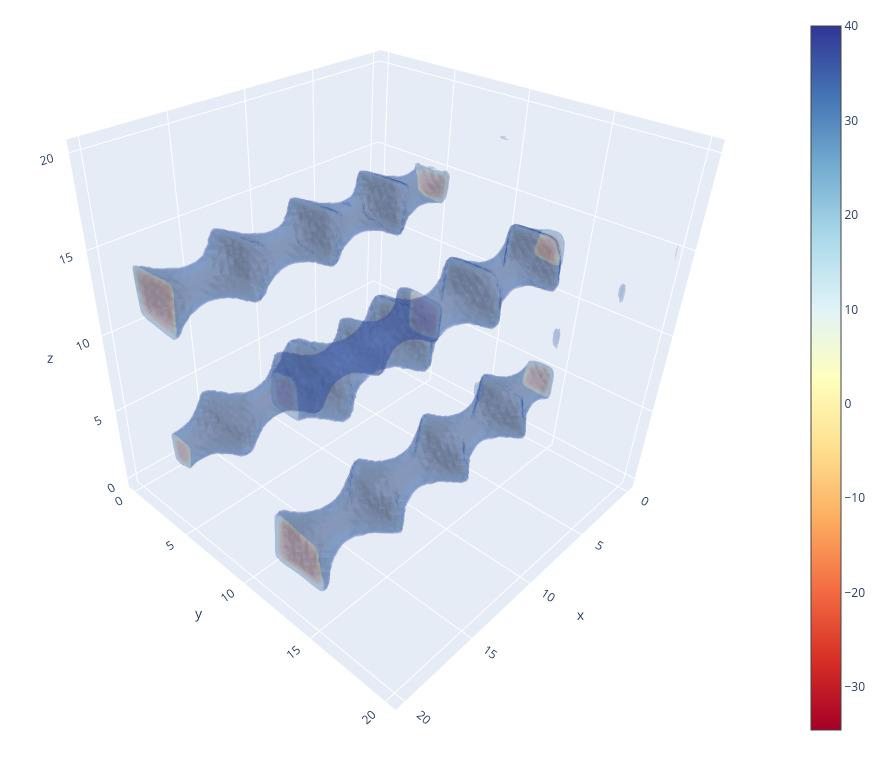
\includegraphics[width=\textwidth]{figures/5-diffusion/viz/XUNSOQ.jpg}
      \caption{XUNSOQ~\cite{Abrahams_2014}}\label{fgr:tube_cavities_a}
  \end{subfigure}
  \hfill
  \begin{subfigure}[b]{0.3\textwidth}
      \centering
      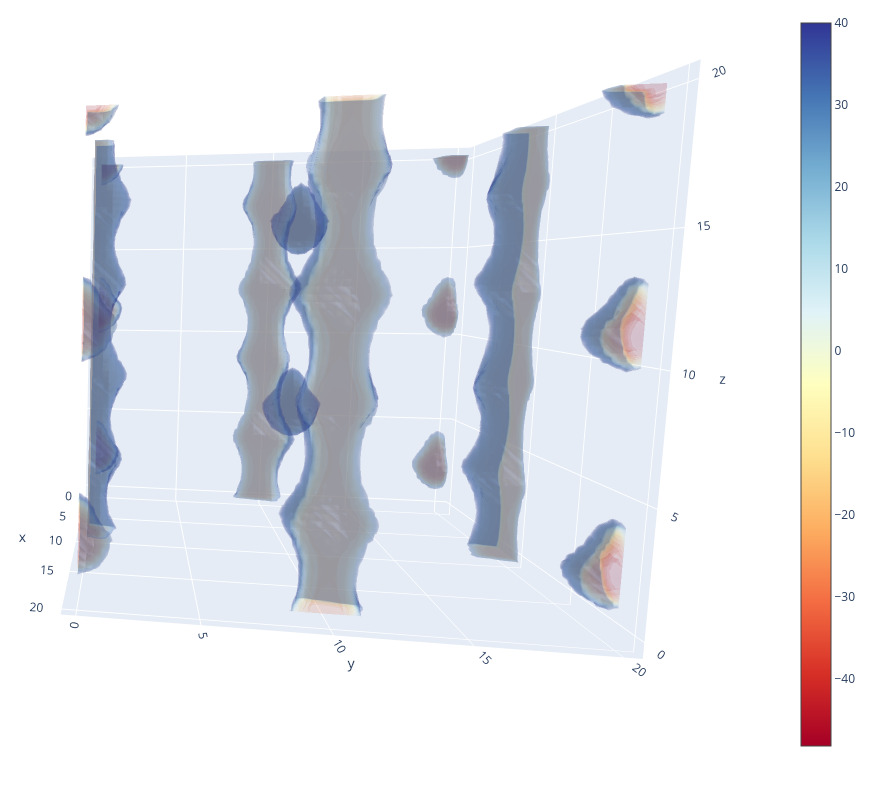
\includegraphics[width=\textwidth]{figures/5-diffusion/viz/BAEDTA01.jpg}
      \caption{BAEDTA01~\cite{Chen_2010}}\label{fgr:tube_cavities_b}
  \end{subfigure}
  \hfill
  \begin{subfigure}[b]{0.3\textwidth}
      \centering
      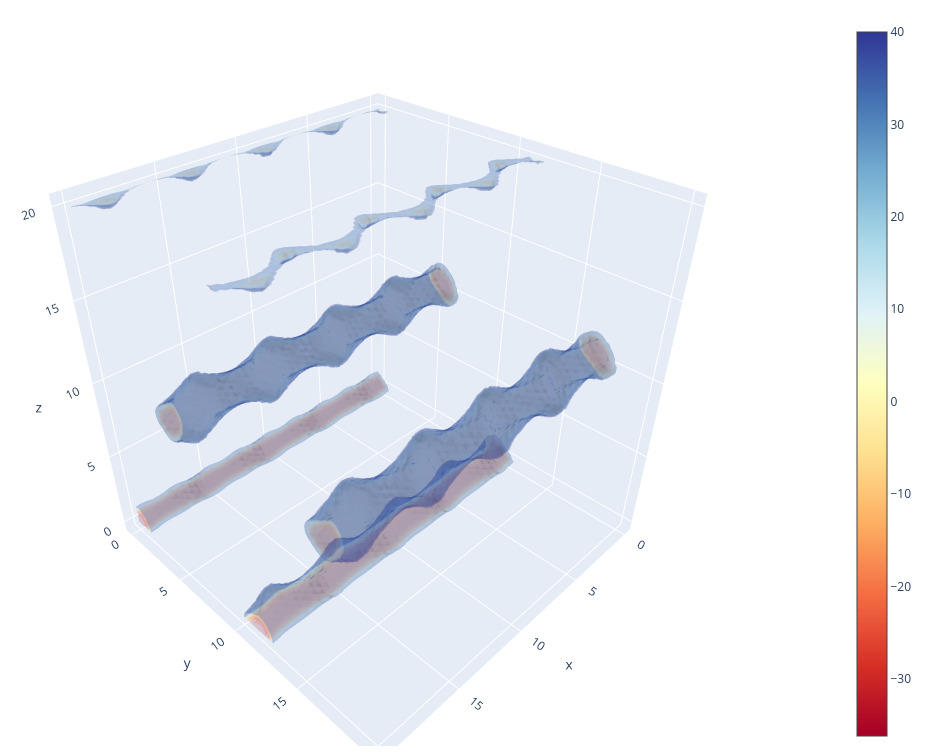
\includegraphics[width=\textwidth]{figures/5-diffusion/viz/TONBII.jpg}
      \caption{TONBII~\cite{Du_2010}}\label{fgr:tube_cavities_c}
  \end{subfigure}
     \caption{ 3D volume plot of the xenon interaction energy values inside materials with non tortuous unidimensional channels calculated using an energy grid as previously described.}\label{fgr:tube_cavities}
\end{figure}

Beyond consideration on the pure diffusion properties, the rather high adsorption selectivity coupled with very little diffusion limitations, make these materials extremely interesting for further study. The material BAEDTA01 has already been mentioned in the study on the selectivity drop due to pressure condition changes, the Figure~\ref{fgr:tube_cavities_b} sheds a brighter light on the origins of this selectivity drop, we can clearly see the two different adsorption sites (one narrower than the other) --- the narrower site is the one giving the very high low-pressure selectivity. The other two materials TONBII and XUNSOQ have a rather stable selectivity value between the low pressure and the ambient pressure cases. If we compare to the KAXQIL structure given by a previous high-throughput screening~\autocite{Simon_2015}, the diffusion coefficients are much higher and the problem of a potential diffusion limitation is solved, the selectivity values of these materials are however yet to be confirmed. The value of the PLD is of course the main factor that explains the lower diffusion coefficient of KAXQIL, but for similar values of PLD, the LCD-PLD difference can be a secondary variable that helps distinguish materials with similar PLD values but different diffusion coefficients. 


If we now look at the other materials, as we can see of the Figure~\ref{fgr:zigzag}, the channels are much more tortuous than the previous type of channel. It seems to make a ``zig-zag'' like shape. On this little amount of data, it is hard to quantify the effect of the tortuosity on the diffusion coefficient --- to do so we would need to compare very similar materials (same chemical nature, same pore size) but has only a difference in tortuosity. Howerver, in a theoretical point of view, the tortuosity usually has a negative effect on the diffusion coefficients. VOHQIS, for instance, has a high degree of tortuosity as shown on the Figure~\ref{fgr:zigzag_a}, and the diffusion properties are not very high, but it is hard to disentangle the effect of the pore size (very big difference between LCD and PLD) from the effect of the tortuosity. A more quantitative approach should be adopted to bring more insights on the diffusion process in nanoporous materials. 

\begin{figure}[ht]
  \centering
  \begin{subfigure}[b]{0.3\textwidth}
      \centering
      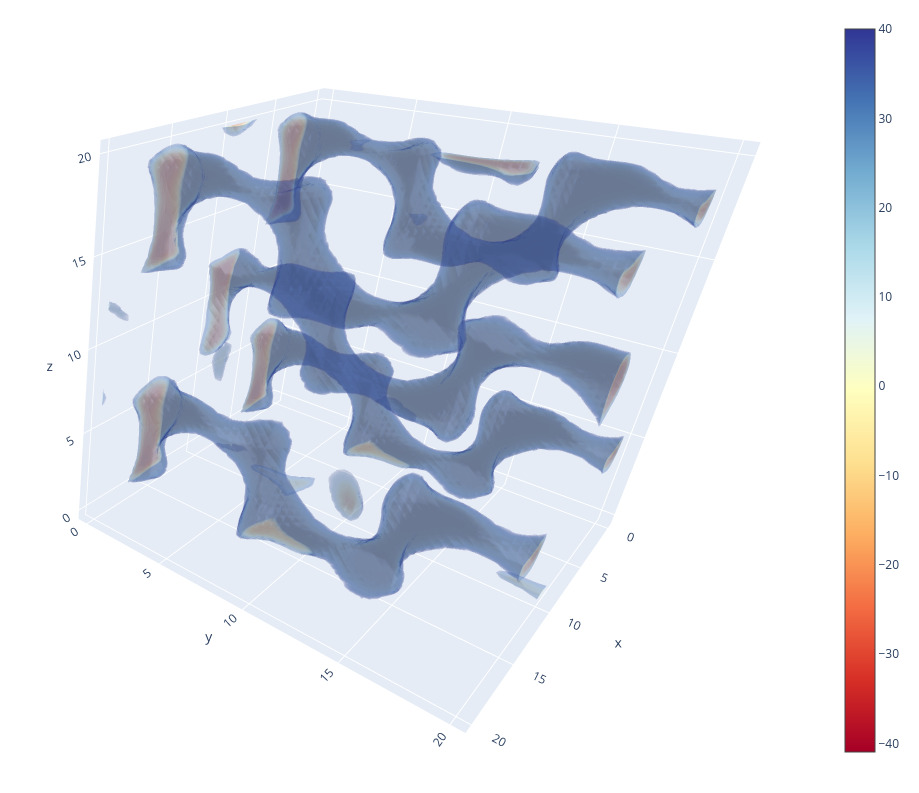
\includegraphics[width=\textwidth]{figures/5-diffusion/viz/VOHQIS.jpg}
      \caption{VOHQIS~\cite{Wragg_2001}}\label{fgr:zigzag_a}
  \end{subfigure}
  \hfill
  \begin{subfigure}[b]{0.3\textwidth}
      \centering
      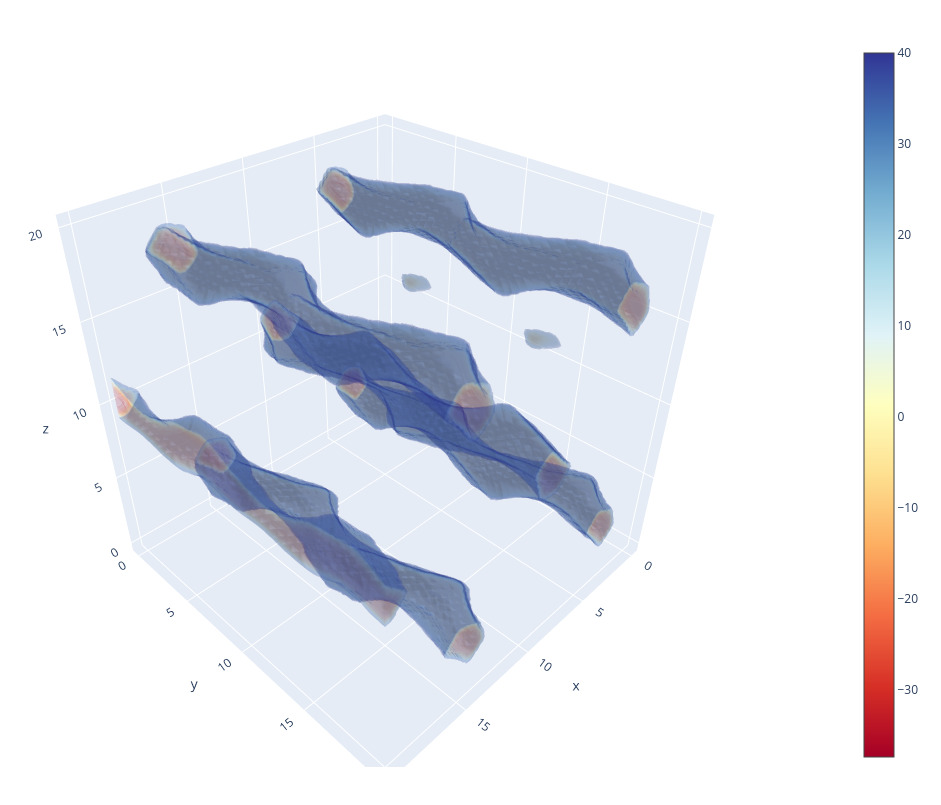
\includegraphics[width=\textwidth]{figures/5-diffusion/viz/GUMDEZ.jpg}
      \caption{GUMDEZ~\cite{Yin_2014}}\label{fgr:zigzag_b}
  \end{subfigure}
  \hfill
  \begin{subfigure}[b]{0.3\textwidth}
      \centering
      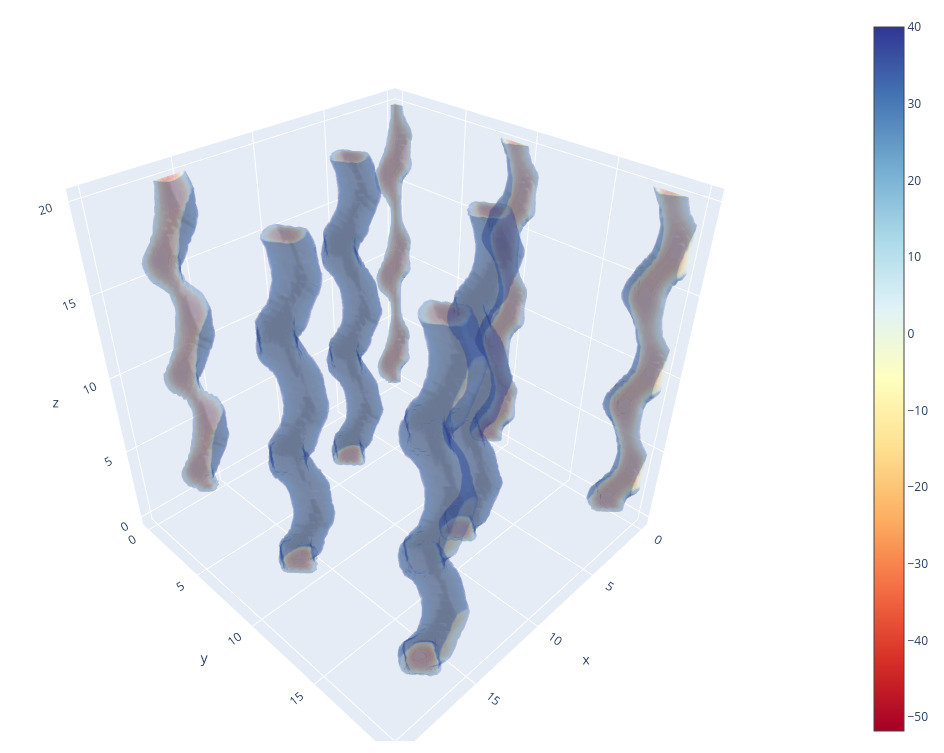
\includegraphics[width=\textwidth]{figures/5-diffusion/viz/MISQIQ.jpg}
      \caption{MISQIQ~\cite{Tong_2013}}\label{fgr:zigzag_c}
  \end{subfigure}
     \caption{ 3D volume plot of the xenon interaction energy values inside materials with tortuous unidimensional channels calculated using an energy grid as previously described.}\label{fgr:zigzag}
\end{figure}

If make a similar analysis for these materials than for the previous materials with strainght channels, there seem to be the same --- it is not surprising since these materials are included in the correlation plot on the Figure~\ref{fgr:porediff_c}. GUMDEZ is much less tortuous as shown on the Figure~\ref{fgr:zigzag_b}, but the difference in tpore size is also lower, the diffusion coefficient is therefore higher, which explains the good diffusion selectivity. This material also has a much higher xenon uptake than more selective materials like KAXQIL, this is due to the notion uptake--selectivity trade-off I introduced on the Figure~\ref{fgr:sa} for instance. For this reason, this material along with QOZDOY was also previously identified in the literature by the xenon/krypton separation screening made by Chung et al.\autocite{Chung_2019} when introducing the CoRE MOF 2019 database. These materials were presented as having a high xenon/krypton selectivity and much higher xenon uptake, which is also a key metric for industrial separation process --- it typically sets how much xenon can be retrieved per adsorption-desorption cycle. To complexify, the screening I could also add an optimization of the xenon uptake to optimization of the diffusion and selectivity properties. By chance, I found materials such as XUNSOQ, QOZDOY qnd GUMDEZ with good adsorption selectivity, diffusion selectivity and xenon uptake that could be much more versatile than very specialized materials such as KAXQIL. 

To sum-up, I performed a screening of diffusion properties for xenon and krypton to inform the previous purely thermodynamic properties screening and I found materials with a good balance between bothe diffusion and adsorption selectivity values. Some of these materials also exhibit very high Xe uptake, which could improve the productivity of xenon in a separation process in addition to a high separative capacity and a fast penetration of the gas inside the material. This study further justifies the mutivariate nature of the optimization problem when looking for a good material for xenon/krypton separation --- it is not sufficient to only look at a single variable. This study brings a more exhaustive approach than already existing studies (on other systems) on the importance of kinetic effects in an adorption process.\autocite{Stanton_2022}
There are still some work to do on a finer comprehension between the diffusion properties and tortuosity and all the pore size effects. The next section will be dedicated to developping faster methodologies of the screening of transport properties so that I can scale the screening methodology to larger databases. To achieve faster transport property screening, I explored methods based on the transition state theory and machine learning prediction models.

\section{Fast diffusion calculation algorithm}\label{sct:algo_diff}

To go beyond the very computationally demanding MD simulation, in this section, I will present alternative methods that I developed during my thesis to calculate the diffusion coefficient. For instance, methods based on the transition state theory can more efficiently generate MSD at larger time-scales. If we apply a similar algorithm as in TuTraST, we can also overcome the initialization problem of MD simulation when different channels are available in an automated screening --- of course it is always possible to manually put the particle in a given initial state, but it is hard to achieve in a screening process. At this stage of my work, I did not finish the implementation of the C++ algorithm that directly reproduces diffusion coefficients through a rejection-free lattice kinetic Monte Carlo algorithm. However, I used the initial implmentation to calculate maximum barrier energy inside a material. This barrier energy was found to bring a complementary information to the PLD values to predict the diffusion coefficient, and an ML model was trained to predict diffusion coefficients much faster than the current MD method.

\subsection{Planned algorithm for TS detection}

I used the GrAED algorithm presented on section~\ref{sct:grid} to calculate the xenon interaction energy with the material at each non-overlapping point of the symmetry-aware grid. With this energy grid, it is now possible to identify the different channels, adsorption pores and the transition surface that separate them. 

I changed a little bit the approach previously described in the section~\ref{sct:tutrast} and adopted by Mace et al.\ to identify the three main components of the lattice Monte Carlo approach. Instead of detecting the channels on the fly, I decided to detect the channels before-hand in order to restrict the cluster growth to a specific channel. This will help decreasing the computation time required during this clustering step since we can do the simulation only for one representing channel out of all the potentially equivalent channels --- because of the high order of symmetry, there are usually equivalent channels within a single unit cell, as shown on the Figures~\ref{fgr:tube_cavities} and~\ref{fgr:zigzag}. 

To identify the different channels, I used a breadth-first search algorithm to find all connected grid points with energy below a given energy threshold value $E\e{cutoff}$. The connection is defined using the faces of the grid voxel, there are 6 such neighbors. Connections from the 8 edges can be added, and we end up with 14 nearest neighbors. If we add the vertices, we can go up to 26 nearest neighbors. To keep things simple, we only used the 6 obvious connections. The breadth-first search algorithm in a grid system is rather pretty simple:

We loop over all the points of our grid:
  \begin{enumerate}
    \item if the point is not already visited and the energy is below the threshold, then the point is saved in the cluster and to a queue, and a search can be initiated to find all the connected neighbors. 
    \item each (face-connected) neighbor of the point is tested, and is added to the cluster and to a queue if it is not already visited and the energy is below the threshold.
    \item we repeat the process for every single elements of the queue until the queue becomes empty. At the en we end-up with all the grid points connected to the initial grid point. Then the main loop restarts, and the search restarts only if we find a point that has not yet been visited.
  \end{enumerate}
At the end of the breadth-first search we end up with clusters of connected points that are below a given energy threshold. Each of these clusters, can be tested to see if they are actually channels (connected all the way through a periodic boundary). 

Now that we have well-defined channels and pockets of our nanoporous material, we can identify the symmetrically equivalent channels by using our symmetrical grid as already explained in the section~\ref{sct:grid}. Then, we usually end up with a few unique channels (less than three in most cases) that can be used for the basin-cluster growth and the detection of TS surfaces that separate these basins. 

Then, we will need to loop over the energy values (in the original paper a step of \SI{1}{\kJ\per\mole} is used), and grow the cluster layer by layer. At this point of the development, another point of improvement is added, I used the previous serach algorithm to quickly count the number of clusters wthin a given channel. If this number changes, it means that some clusters merged. If the energy gap is high enough, we can start to detect the TS surfaces using a layer-by-layer growth within a small energy range ($[E,E+\delta E]$) to generate a smoother surface. 

I am currently at the last step of the development of this detection algorithm, because the development was put in stand-by to focus on the analysis of the barrier energies calculated from a modified version of this first implementation, which will be detailed in the following discussions. The transition surface detection will be further discussed in the next chapter, and I will try to implement a more optimized version of this detection that could avoid using a computationally expensive layer-by-layer growth. 

\subsection{Calculation of diffusion activation energy}

Since we only want to determine the activation energy, we can skip the more computationnally demanding TS detection and kinetic Monte Carlo steps. To do so we can simply use the breadth-first search algorithm to label the different connected components inside a given channel between $E\e{min}$ and $E\e{min}+i\delta E$ (at the $i$\ex{th} iteration). When the number of connected components changes between two energy values $E$ and $E+\delta E$, there are new components appearing or old components that merged or both happening at the same time. By looking at the number of connected components, the code automatically detects the energy $E\e{barrier}$ at which the components connect back together and form a channel (possibility to go from one boundary to another). This energy corresponds to the energy required to be able to diffuse through a channel. Then, the activation energy $E\e{a}$ simply corresponds to the difference between this barrier energy $E\e{barrier}$ just calculated and the minimal energy $E\e{min}$ within the channel. 

In the case of KAXQIL, we can carry out a barrier detection using an energy step $\delta E$ of \SI{0.3}{\kJ\per\mol}. There is only one symmetrically unique type of channel in KAXQIL with a minimal energy of $-44.3$~\si{\kJ\per\mole} --- the different channels shown on the Figure~\ref{fgr:KAXQIL_channel} are all symmetrically equivalent. The code only detects one merge that leads to an all connected component inside the channel. This merge occurs for an energy of $-25.7$~\si{\kJ\per\mole} (as shown on the Figure~\ref{fgr:KAXQIL_23}), which means that the activation energy is estimated to be $18.6$~\si{\kJ\per\mole} with an error of \SI{0.3}{\kJ\per\mole} (due to the energy step considered). 

\begin{figure}[ht]
  \centering
  \begin{subfigure}[b]{0.3\textwidth}
    \centering
    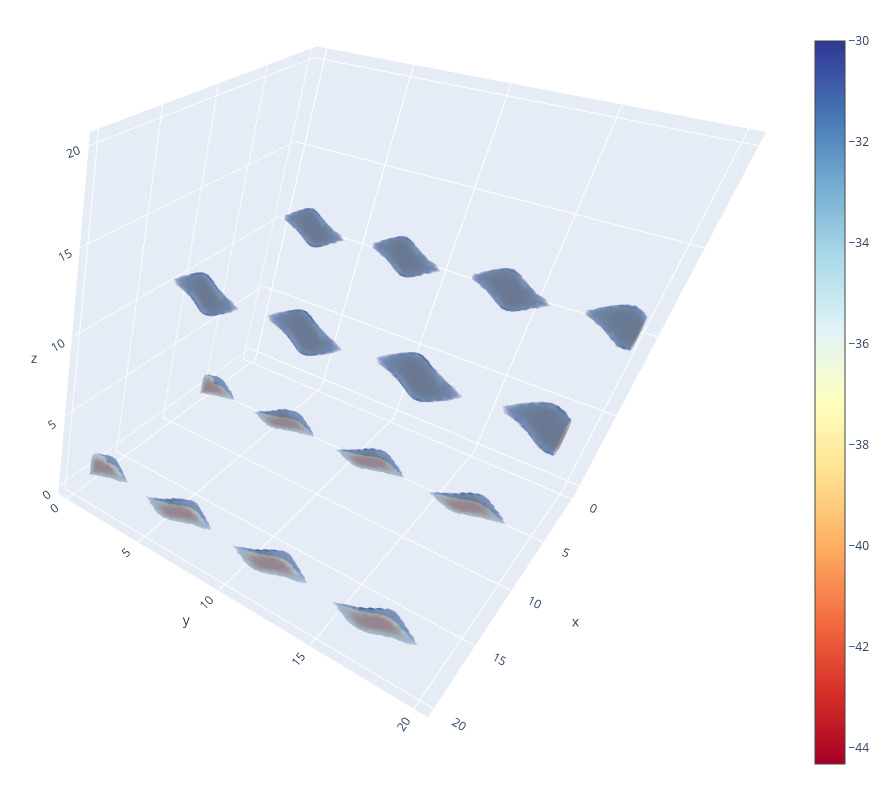
\includegraphics[width=\textwidth]{figures/5-diffusion/KAXQIL_30.jpg}
    \caption{$E\e{max}<-30$}~\si{\kJ\per\mole}\label{fgr:KAXQIL_30}
  \end{subfigure}
  \hfill
  \begin{subfigure}[b]{0.3\textwidth}
    \centering
    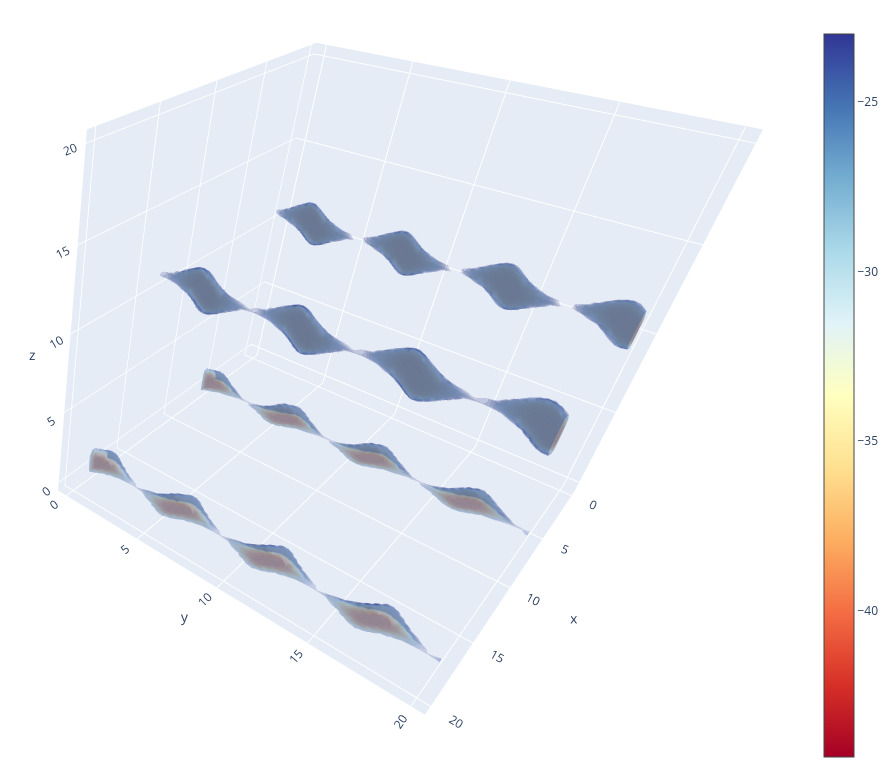
\includegraphics[width=\textwidth]{figures/5-diffusion/KAXQIL_23.jpg}
    \caption{$E\e{max}<-23$}~\si{\kJ\per\mole}\label{fgr:KAXQIL_23}
  \end{subfigure}
  \hfill
  \begin{subfigure}[b]{0.3\textwidth}
      \centering
      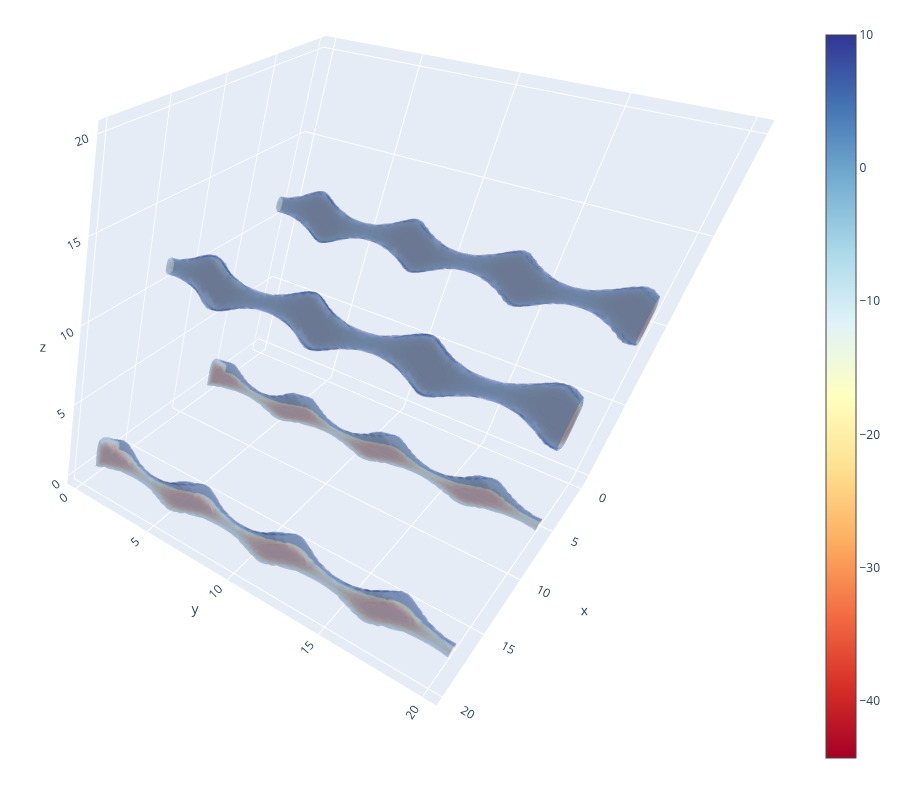
\includegraphics[width=\textwidth]{figures/5-diffusion/KAXQIL_10.jpg}
      \caption{$E\e{max}<10$}~\si{\kJ\per\mole}\label{fgr:KAXQIL_channel}
  \end{subfigure}
    \caption{ 3D visualization of channels within KAXQIL using different energy thresholds $E\e{max}$. Depending on the maximum value of energy allowed, the channel is either composed of unconnected basins (a), or they are fully connected (b) and (c). This illustrates the principle of the barrier energy detection. }\label{fgr:KAXQIL_channels}
\end{figure}

In this simple case of one unique merge of a unidimensional channel, the method works pretty well and it is possible to associate this activation energy to a diffusion rate $k\e{diff}$ using the Arrhenius equation:
\begin{equation}
  k\e{diff} = A \exp\left(-\frac{E\e{a}}{k\e{B}T}\right)
\end{equation}
where $A$ is a prefactor that depend on the temperature and the system (adsorbate, adsrobent). This is a simplified version of the equations~\ref{eq:trans_rate_path} and~\ref{eq:trans_rate} used in transition state theory-based methods. In the case of a unidimensional channel with only one transition possible, the diffusion coefficient is directly related to the diffusion rate. The problem can be reduced to a unidimensional random walk with a given transition probability, and the diffusion coefficient is then simply $D=0.5k\e{diff}L^2$ where $L$ is the distance between two basins (in one dimension). We end up in this special case with a direct relation between the diffusion coefficient and the activation energy $\log(D)\propto E\e{a}$.
If we consider more complex systems than KAXQIL, this methods may not work that well. 

The case of multistep diffusion is much harder to describe, for example --- a particle can cross a series of lower barrier instead of making the highest energy gap (calculated by our method) as illustrated on the Figure~\ref{fgr:TS_problem}. In this particular case, the relevant activation energy is in fact the maximum value between these two activation energies. And even if we take the maximum activation energy, in the case where they are similar in value, this approximation can be unjustified. Both transitions would influence the diffusion. This approximation is only true if one af the activation energy is much larger than the other ($E\e{a}^1 \gg E\e{a}^2$).

\begin{figure}[ht]
  \centering
    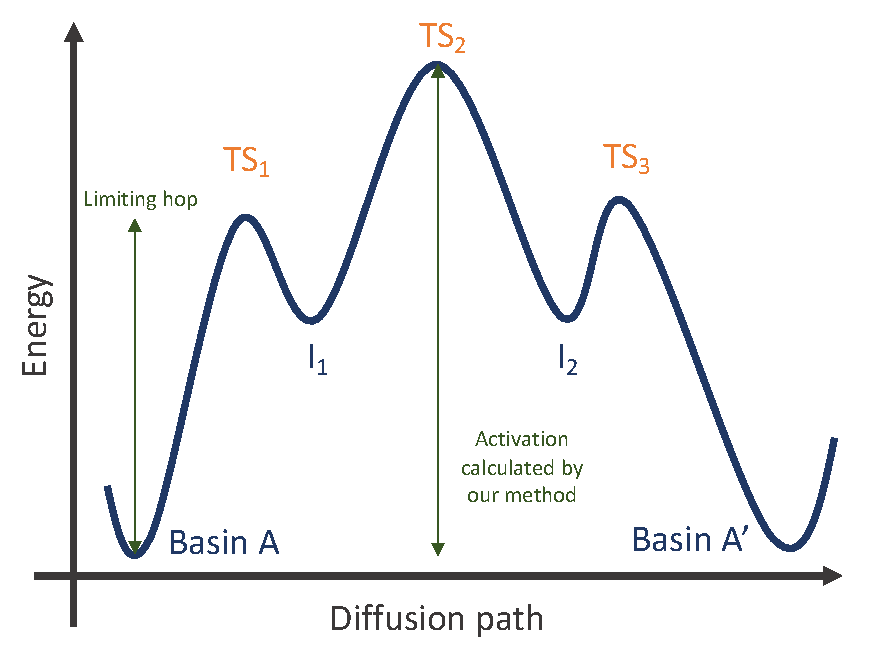
\includegraphics[width=0.6\textwidth]{figures/5-diffusion/Diffusion_TS.pdf}
    \caption{Multi-step diffusion from a basin A to a basin A'. The diffusion process is modeled by transition states TS$_1$, TS$_2$ and TS$_3$ and intermediate steps I$_1$ and I$_2$. In this particular case, there is a difference between the real limiting activation energy and the activation energy calculated by our simplified method. }\label{fgr:TS_problem}
\end{figure}

To improve this approach,we could detect intermediate transition state energy values by looking at the change in the number of clusters for instance. But again it is hard to say which combinations of energy difference are relevant, and more detailed investigation of the location of these transition states are needed, which is the initial problem of TS surface detection that we put on stand-by. Aware of all these weaknesses, we can however use this quickly measurable activation energy as a proxy of the diffusion coefficient. 
This will be the object of the next discussion on the relation between this approximated activation energy value and the diffusion coefficients. This new diffusion desriptor can later be used in prediction models as a complementary descriptor to the PLD to give a more complete picture of the diffusion process. 

\subsection{Relation of the approximated activation energy to the diffusion coefficient}


I calculated this xenon diffusion activation energy for all the 5,125 structures selected for the xenon diffusion coefficient screening presented in the section~\ref{sct:xenon_diff_screen}. I used a $\delta E$ of \SI{0.1}{\kJ\per\mol} for the loop over the energies to find the minimal barrier energy of each unique channels of the material. An activation energy can then be deduced and compared to the diffusion coefficeints. To avoid any noise that could come from the MD simulation initialization problem, we removed all the materials with very different barrier energy values from one channel to the other (the standard deviation of the barrier energy values is higher than \SI{1}{\kJ\per\mol}). These materials only represent 145 materials out of 5,125.


\begin{figure}[ht]
  \centering
  \begin{subfigure}[b]{0.48\textwidth}
    \centering
    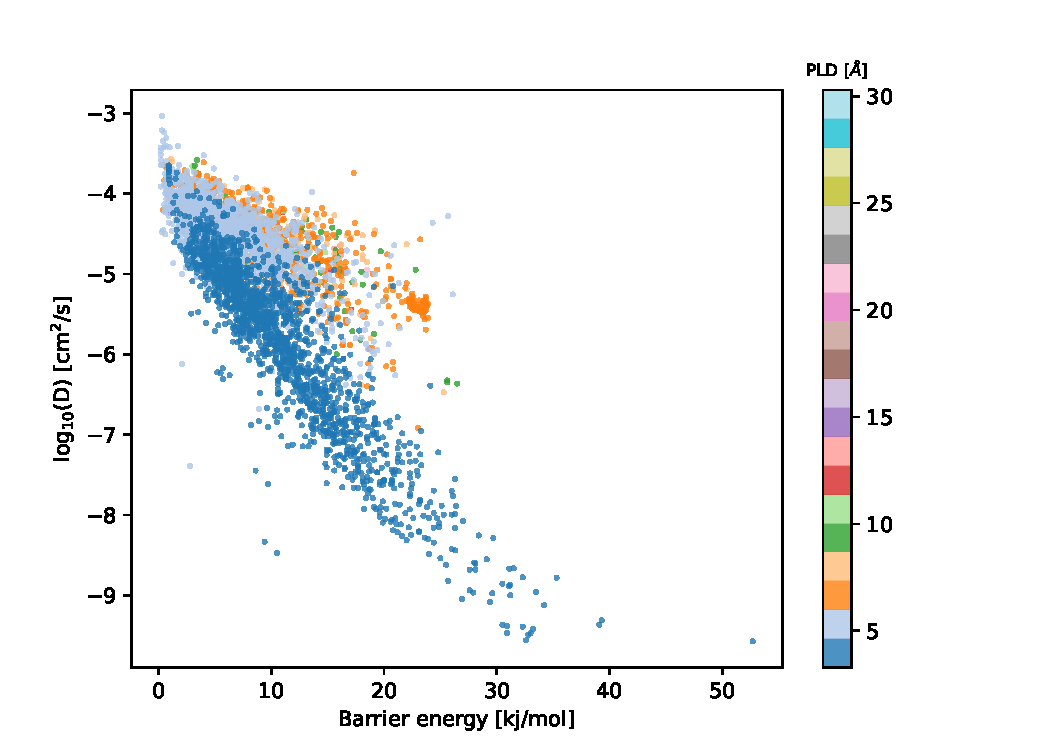
\includegraphics[width=\textwidth]{figures/5-diffusion/difflog_barrier_Df_uff.pdf}
    \caption{All structures}\label{fgr:barrier_diffusion_a}
\end{subfigure}
  \hfill
  \begin{subfigure}[b]{0.48\textwidth}
      \centering
      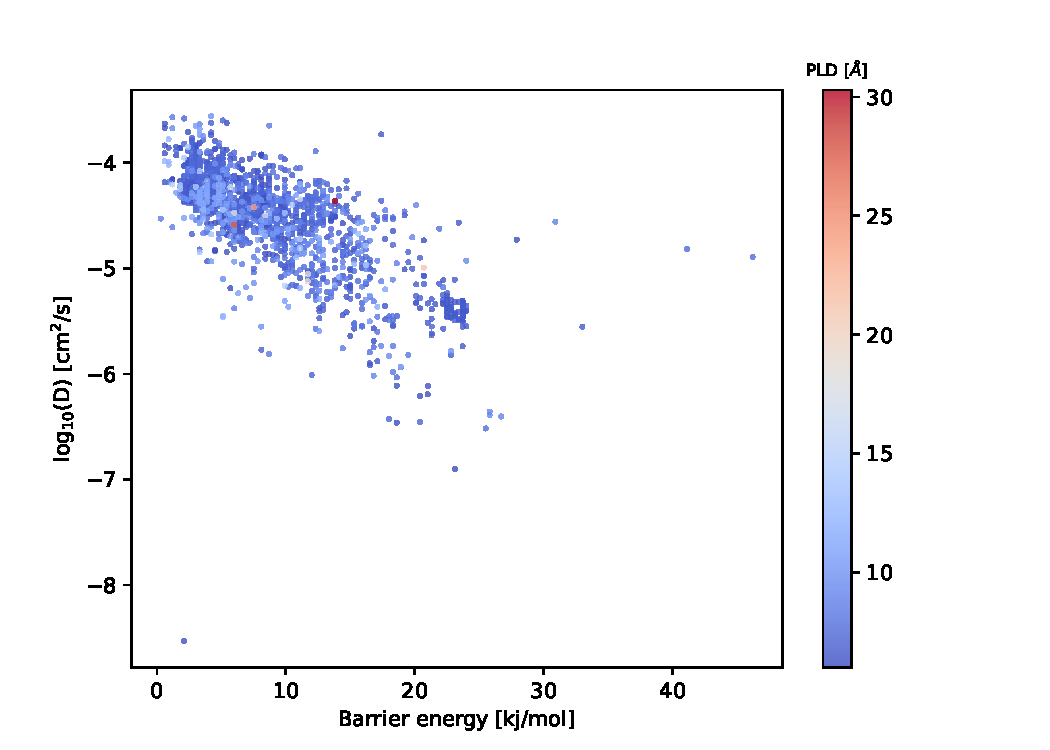
\includegraphics[width=\textwidth]{figures/5-diffusion/difflog_barrier_Df_uff_2.pdf}
      \caption{PLD over \SI{6}{\angstrom}}\label{fgr:barrier_diffusion_b}
  \end{subfigure}
    \caption{ \todo{}}\label{fgr:barrier_diffusion}
\end{figure}

As shown on the Figure~\ref{fgr:barrier_diffusion_a}, the activation energy is correlated to the diffusion coefficient for xenon. The correlation seems to be much stronger for the points with a PLD around \SI{4.5}{\angstrom}, and for PLD values over \SI{6}{\angstrom}, there still is a correlation but it seems weaker than for smaller values of PLD as shown by the Figure~\ref{fgr:barrier_diffusion_b}

This correlation between the barrier energy and the diffusion coefficient is confirmed on the Figure~\ref{fgr:diff_pld_barrier}. The points are labeled according to the barrier energy value, and the highest barrier energy points are mostly concentrated on lower values of diffusion coefficient. We can, however, see some very high barrier energy points associated to points with quite low diffusion coefficient, there are two such points detectable with our bear eyes. 

\begin{figure}[ht]
  \centering
    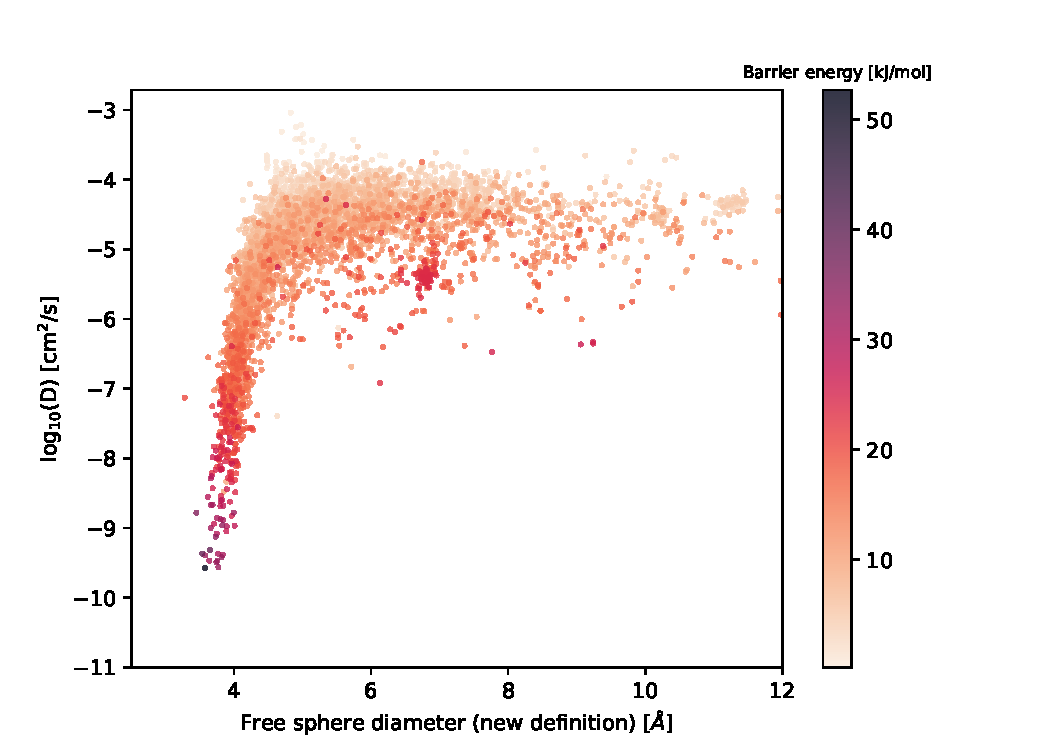
\includegraphics[width=0.6\textwidth]{figures/5-diffusion/difflog_Df-uff298K_barrier.pdf}
    \caption{\todo{change the xlabel}}\label{fgr:diff_pld_barrier}
\end{figure}

This barrier activation energy descriptor completes the description of the diffusion coefficient given by PLD values. As discussed in the dedicated section, the PLD values can not distinguish between the structures over \SI{6}{\angstrom} in the ``plateau'', and the difference of diffusion coefficient could only be considered as noise in the previous analysis. But it seems that on the Figure~\ref{fgr:diff_pld_barrier}, the higher values of barrier energies are found for lower diffusion coefficient in the plateau value, hence explaining the different values within the plateau by the value of the activation barrier. 
Although the correlation is not perfect, this barrier descriptor better informs on this uncharted area of PLD values above \SI{6}{\angstrom} impossible to explain with simple geometrical considerations. This barrier activation energy value informs on the chemical nature of the diffusion barrier to be crossed. 

In the final section of this chapter, I will therefore combine geometrical descriptors to this barrier energy to train a machine learning model following the same approach as in the previous chapter 4. The barrier energy and the PLD values are the most correlated descriptors and will play a prominent role in the final ML model. This model could then be used to evaluate the diffusion coefficeint of xenon in other materials, which is much faster than usign MD simulations.

\subsection{ML prediction model}

Diffusion coefficients are extremely time-consuming to calculate and with a lot of complications in the final fitting process. From the 6,525 initial structures, we lost more than a thousand structures, which corresponds to about 79\% success rate due to either a lack of time to give a usable MSD or simply to MSD that describe non-diffusional regimes. By using a rather unconventionally higher time step, we managed to reduce the time required to probe the diffusion regime to only a couple of days per structure. Compared to the \SI{12}{second} required for the barrier energy calculation with an energy step of \SI{0.1}{\kJ\per\mol}, and the few minutes required to run Zeo++, the MD method is extremely slow. If we use very optimistic hypothesis for the MD simulations, we are basically comparing 24 hours to maybe at most 10 minutes per structure, which corresponds to approximately 150-fold speed-up (in reality it is much higher). However, the relationships between the barrier energy, PLD and the diffusion coefficient are not clear --- the arrhenius law generalizes poorly considering the weak correlation shown by the Figure~\ref{fgr:barrier_diffusion_a}. The ML model is here to draw this relation to achieve a good prediction, while spending less time in the future to predict the diffusion coefficient of future selective materials.


\begin{table}[ht]
  \setlength{\extrarowheight}{1pt}
  \centering
  \begin{tabular}{|l|c|m{8cm}|}
  \hline
    Feature name  &  Symbol   &   Description\\
  \hline
      "Framework Mass (g/mol)" &   $M_f$ &   Molar mass of the framework material considered  \\
      "Framework Density (kg/m\^3)" &   $\rho_f$ &   Mass density of the framework material considered  \\
      "ASA\_m2/cm3\_1.2" &   SA &   Surface area accessible to a \SI{1.2}{\angstrom} radius probe in \si{\square\m\per\cubic\cm}  \\
      "PO\_VF\_2.0" &   $V\e{pore}$ &  L2-regularization parameter  \\
      "D\_f\_vdw\_uff298" &   PLD or $D_f$  &   Pore limiting diameter of largest free sphere diameter calculated using the UFF dependent definition  \\
      "D\_if\_vdw\_uff298" &   LCD or $D_{if}$ &   Largest included free sphere diameter in a free diffusion path calculated using the UFF dependent definition  \\
      "Adsorption\_enthalpy" &   $\Delta\e{ads}H_0\ex{Xe}(\text{channel})$  &   Xenon adsorption enthalpy within a channel calculated using the barrier algorithm  \\
      "barrier\_kjmol" &   $E\e{a}$  &   difference between barrier energy $E\e{barrier}$ and the minimal energy $E\e{a}$ within a channel \\
      "delta\_LCD\_PLD" &   LCD$-$PLD  &   difference between the LCD and PLD values \\
      "1D\_chan" &  $\mathbb{1}\e{1D}$   &   categorial feature: 1 if there is a unidimensional channel, 0 else \\
      "2D\_chan" &  $\mathbb{1}\e{2D}$   &   categorial feature: 1 if there is a bidimensional channel, 0 else \\
      "3D\_chan" &  $\mathbb{1}\e{3D}$   &   categorial feature: 1 if there is a tridimensional channel, 0 else \\
    \hline
  \end{tabular}
  \caption{ Features used in the ML model for diffusion coefficeint prediction }\label{Table:feat_diff}
\end{table}

To train the ML model, I used {80\%} of the 4,873 structures that survived all the different imposed filters. And I used 12 different descriptors described in the Table\ref{Table:feat_diff} to train this model. The hyperparameters of the XGBoost model was determined using a similar approach as in the chapter 4, and the following were used:

\begin{lstlisting}[language=Python]
  optimal_params = {
      'objective': 'reg:squarederror',
      'n_estimators': 1500,
      'max_depth': 4,
      'colsample_bytree': 1,
      'colsample_bylevel': 0.75,
      'subsample': 0.75,
      'alpha': 0.6,
      'lambda': 1,
      'learning_rate': 0.04,
      }
\end{lstlisting}

With this parameterization, this ML model predicts the $\log_{10}$ of the diffusion coefficient (\si{\square\cm\per\s}) with a root mean square error of $0.26$ on the test set and a mean absolute error of $0.18$. This means that the exponent $\alpha$ is known with an error of about $0.2$ if we express the diffusion coefficient as $D = 10^{\alpha}$. As a point of comparison the previous ML model for thermodynamic selectivity predicts the $\log_{10}$ of the selectivity with an error of about $0.07$. Here, we are not trying to predict the exact values of the diffusion coefficient as there is already a lot of noise in the values generated by MD simulation (about {20\% relative error for KAXQIL}), but we rather try to determine the order of magnitude of the diffusion coefficient value. This model achieves just that, as illustrated on the Figure~\ref{fgr:diffusion_pred}, the predicted diffusion coefficient is very close to the true value in a log scale representation.


\begin{figure}[ht]
  \centering
    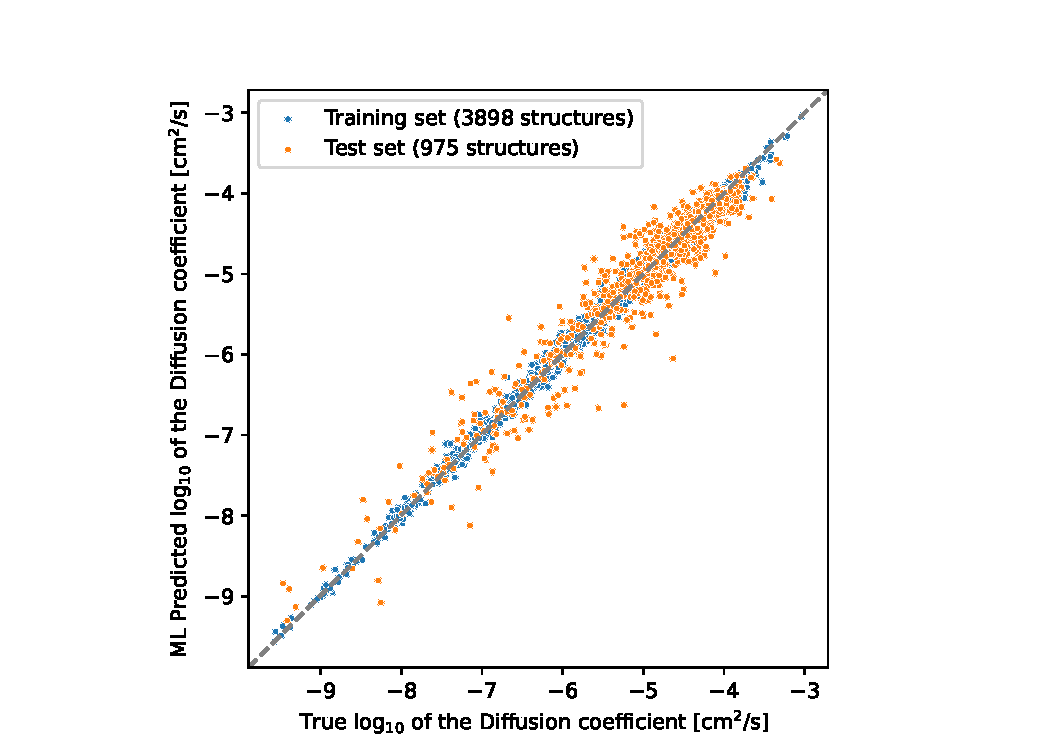
\includegraphics[width=0.48\textwidth]{figures/5-diffusion/diffusion_prediction.pdf}
    \caption{ \todo{}}\label{fgr:diffusion_pred}
\end{figure}

\todo{Stability training}

\todo{dependence plot}





\section{Beyond self-diffusion screenings}

In this chapter, I introduced different methods of evaluating the transport properties of an adsorbate inside a nanoporous material. The most accurate method requires much more computational time and personal attention to achieve the best accuracy. For instance, we need to choose carefully the parameters of the MD simulation so that we obtain a mean square displacement data relevant for diffusion coefficient calculation. I managed to perform a screening of diffusion coefficient values for xneon and krypton to find interesting materials that exhibit both good thermodynamic and kinetic separation performance. These values have also been used to serve as a baseline data to test out other methods such as the activation energy detection and an ML model. The final ML model seems to give very promising performance by achieving a root mean square error of only $0.25$ \todo{recheck} on the base-10 logarithm of the diffusion coefficient. This means that we can evaluate quite accurately the order of magnitude of the diffusion properties. This could help quickly identify possible diffusion limitations of a promising material, but also optimize this property for faster equilibration in an adsoprtion based separation. Beyond our study, the techniques developed and to be developed in my work can also apply to membrane separation processes.

Different follow-up studies can be initiated considering the results obtained. For instance, the effect of tortuosity on the diffusion coefficient values and finding relevant ways of defining it remain open questions. We can for example focus on unidimensional channels, where each change of direction can be analyzed to quantify how frequently it appears and the magnitude of the change of direction it makes.\autocite{Bullitt_2003} Another challenge could be measuring different diffusion regimes such as the single-file diffusion that leads to an MSD that has a square root time relation\todo{cite}. The materials with MSD relations other than linear were in fact discarded in this study since I only took materials with high determination coefficients in the linear fit. 

To go beyond standard studies, we can even use the diffusion coefficeint to model the breakthrough experiments which is the closest a lab experiment can get from the industrial adsorption process. The recent development of the RUPTURA software,\autocite{Sharma_2023} enables much more perspectives in the field of modeling. We can for instance calculate the axial dispersion coefficient used in a breakthrough model using transport properties while also injecting the thermodynamic data we have on the adsorption process of xenon and krypton. This gives a real opportunity for experiment-theory comparison in order to start a virtuous feedback loop to improve modeling and help in discovring better materials. 

The diffusion coefficient calculated by the above-mentioned methodologies are by definition only describing a self-diffusion in an infinitely diluted environment. To better describe the transport properties in industrial conditions, we need to study the diffusion coefficients in a higher loading environment to take account of host--host interactions. Furthermore, we can also directly run mixture simulations to retrieve the so-called Onsager diffusion coefficients that are based on the Maxwell-Stefan diffusion equation rather than the Fick's equation.\autocite{Krishna_2008} The calculation of such quantities requires a lot of computational resources since we need to run MD simulations on mixtures at a rather high loading and for long enough in order to capture the diffusion regime. It is therefore unimaginable to apply it in a large-scale screening, but we could consider testing some interesting materials in order to study the mixture and loading effect on the transport properties.

In this chapter, I only presented one aspect that was not taken into account in standard high-throughput screenings for xenon/krypton separation, which is the transport properties. In the next chapter, I will focus on other effects that could help complete the picture in order to be closer to the experimental system. The flexibility of the nanoporous framework can for instance change the adsorption performances.\autocite{Witman_2017} And, the difference in polarizability of xenon and krypton can be better leveraged in the screening procedure if we can properly model it using more high-level theories than the Lennard-Jones potential. Both the flexibility and the polarization are still at the project stage and some results will be presented, but it is mainly a compilation of possible research focuses and solutions that could improve our current understanding. 

\OnlyInSubfile{\printglobalbibliography}

\end{document}